% --------------- PLANTILLA MAXI (GOD) -----------------
\documentclass[11pt, twocolumn]{article}

\usepackage[latin1,utf8]{inputenc}
\usepackage{verbatim}
\usepackage{multirow}
\usepackage{float}
\usepackage{enumerate}
\usepackage{graphics,graphicx,xcolor}
\usepackage{subfig}
\usepackage[spanish,es-tabla]{babel}
\usepackage{caption}
\usepackage{placeins}
\usepackage{afterpage}
\usepackage{blindtext}
\usepackage{multicol}
\usepackage{geometry}
\usepackage{lipsum}

%paquete para referencias
\usepackage[backend=biber, style=nature, citestyle=numeric, sorting=none, maxbibnames=99]{biblatex} % 
% \usepackage{natbib}
% \bibliographystyle{apsrev4-1} % Utiliza el archivo .bst de APS o uno similar

\usepackage{titling} % Paquete para personalizar título del documento
\usepackage{authblk}  % Paquete para personalizar autores del documento
\renewcommand\Authand{ y } % Reemplazar 'and' con 'y'

\DeclareCaptionFormat{custom}
{%
    \textbf{#1#2}\textit{\small #3}
}
\captionsetup{format=custom}

\newgeometry{bottom=3cm, top=2cm, left=3cm, right=3cm}
\usepackage{hyperref}
\hypersetup{
  colorlinks   = true, %Colours links instead of ugly boxes
  urlcolor     = blue, %Colour for external hyperlinks
  linkcolor    = black, %Colour of internal links
  citecolor   = black %Colour of citations
}

%paquete para unidades
\usepackage{siunitx}
% seteo punto como separador decimal
\AtBeginDocument{\decimalpoint}


% \DeclareSIUnit\torr{Torr}

%% Paquetes de la AMS
\usepackage{amsmath, amsthm, amsfonts, amssymb}

%componentes de texto
\usepackage{textcomp}


% Personaliza título del documento
\pretitle{\begin{center}\LARGE\bfseries}
    \posttitle{\par\vspace{0.5em}\end{center}\large}
    \preauthor{\begin{center}\large \lineskip 0.8em \begin{tabular}[t]{c}}
    \postauthor{\end{tabular}\par\end{center}}
    \predate{\begin{center}\large}
    \postdate{\par\end{center}}


\usepackage{fancyhdr}
\pagestyle{fancy}

% Definimos el encabezado de las paginas pares e impares.
\lhead{IMÁGENES MÉDICAS}
\chead{Práctica 3 - 2024}
\rhead{Gatto Maximiliano}
\renewcommand{\headrulewidth}{0.5pt}

% aqui definimos el pie de pagina de las paginas pares e impares.
\lfoot[a1]{}
\cfoot[c1]{\thepage}
\rfoot[e1]{}

\renewcommand{\footrulewidth}{0.5pt}

% ------------------- TITULO ----------------------
% \title{\textbf{Procesamiento de imágenes digitales} \\ \vspace{1cm} \large IMÁGENES MÉDICAS - Práctica 2 - 2024}

\title{{\large IMÁGENES MÉDICAS - Práctica 3 - 2024} \\ \vspace{1cm}\textbf{Reconstrucción de Imágenes Tomográficas: Método Directo}}



\author[ ]{\textbf{Maximiliano Gatto}}
\affil[ ]{Instituto Balseiro (UNCuyo - CNEA) - Bariloche, Río Negro, Argentina\vspace{0.4cm}}
\affil[ ]{\href{mailto:maximiliano.gatto@ib.edu.ar}{maximiliano.gatto@ib.edu.ar}}

\date{\today}

\begin{document}
\maketitle

% ------------------ INTRODUCCION ---------------------
\section{Introducción}


% ------------------ RESULTADOS ---------------------
\section{Resultados}

% --------------- EJ 1 ---------------------
\subsection*{Ejercicio 1}
Se utilizó el fantoma de \textit{Shepp-Logan} rasterizado, presente en el modulo \href{https://scikit-image.org/docs/stable/api/skimage.data.html}{\texttt{data}} de la librería \href{https://scikit-image.org}{\texttt{skimage}} en \texttt{Python}. Las funciones de la librería \texttt{skimage} asumen que el número de detectores $N_D$ es igual al ancho de la imagen, por lo que se optó por reescalear la imagen para cambiar el número de detectores. Para el análisis de los siguientes ejercicios, se estableció que la imagen fue adquirida por $160$ detectores (se utilizó arbitrariamente esta convención en los ejercicios que no requieran un número específico de detectores). 

Se implementó una ecualización del histograma con el algoritmo desarrollado en la \textit{Práctica 1}. El resultado tanto de la imagen original como la ecualizada se muestran en la Figura \ref{fig:figuras_ej_1}

\begin{figure}[H]
    \centering
    \subfloat[]{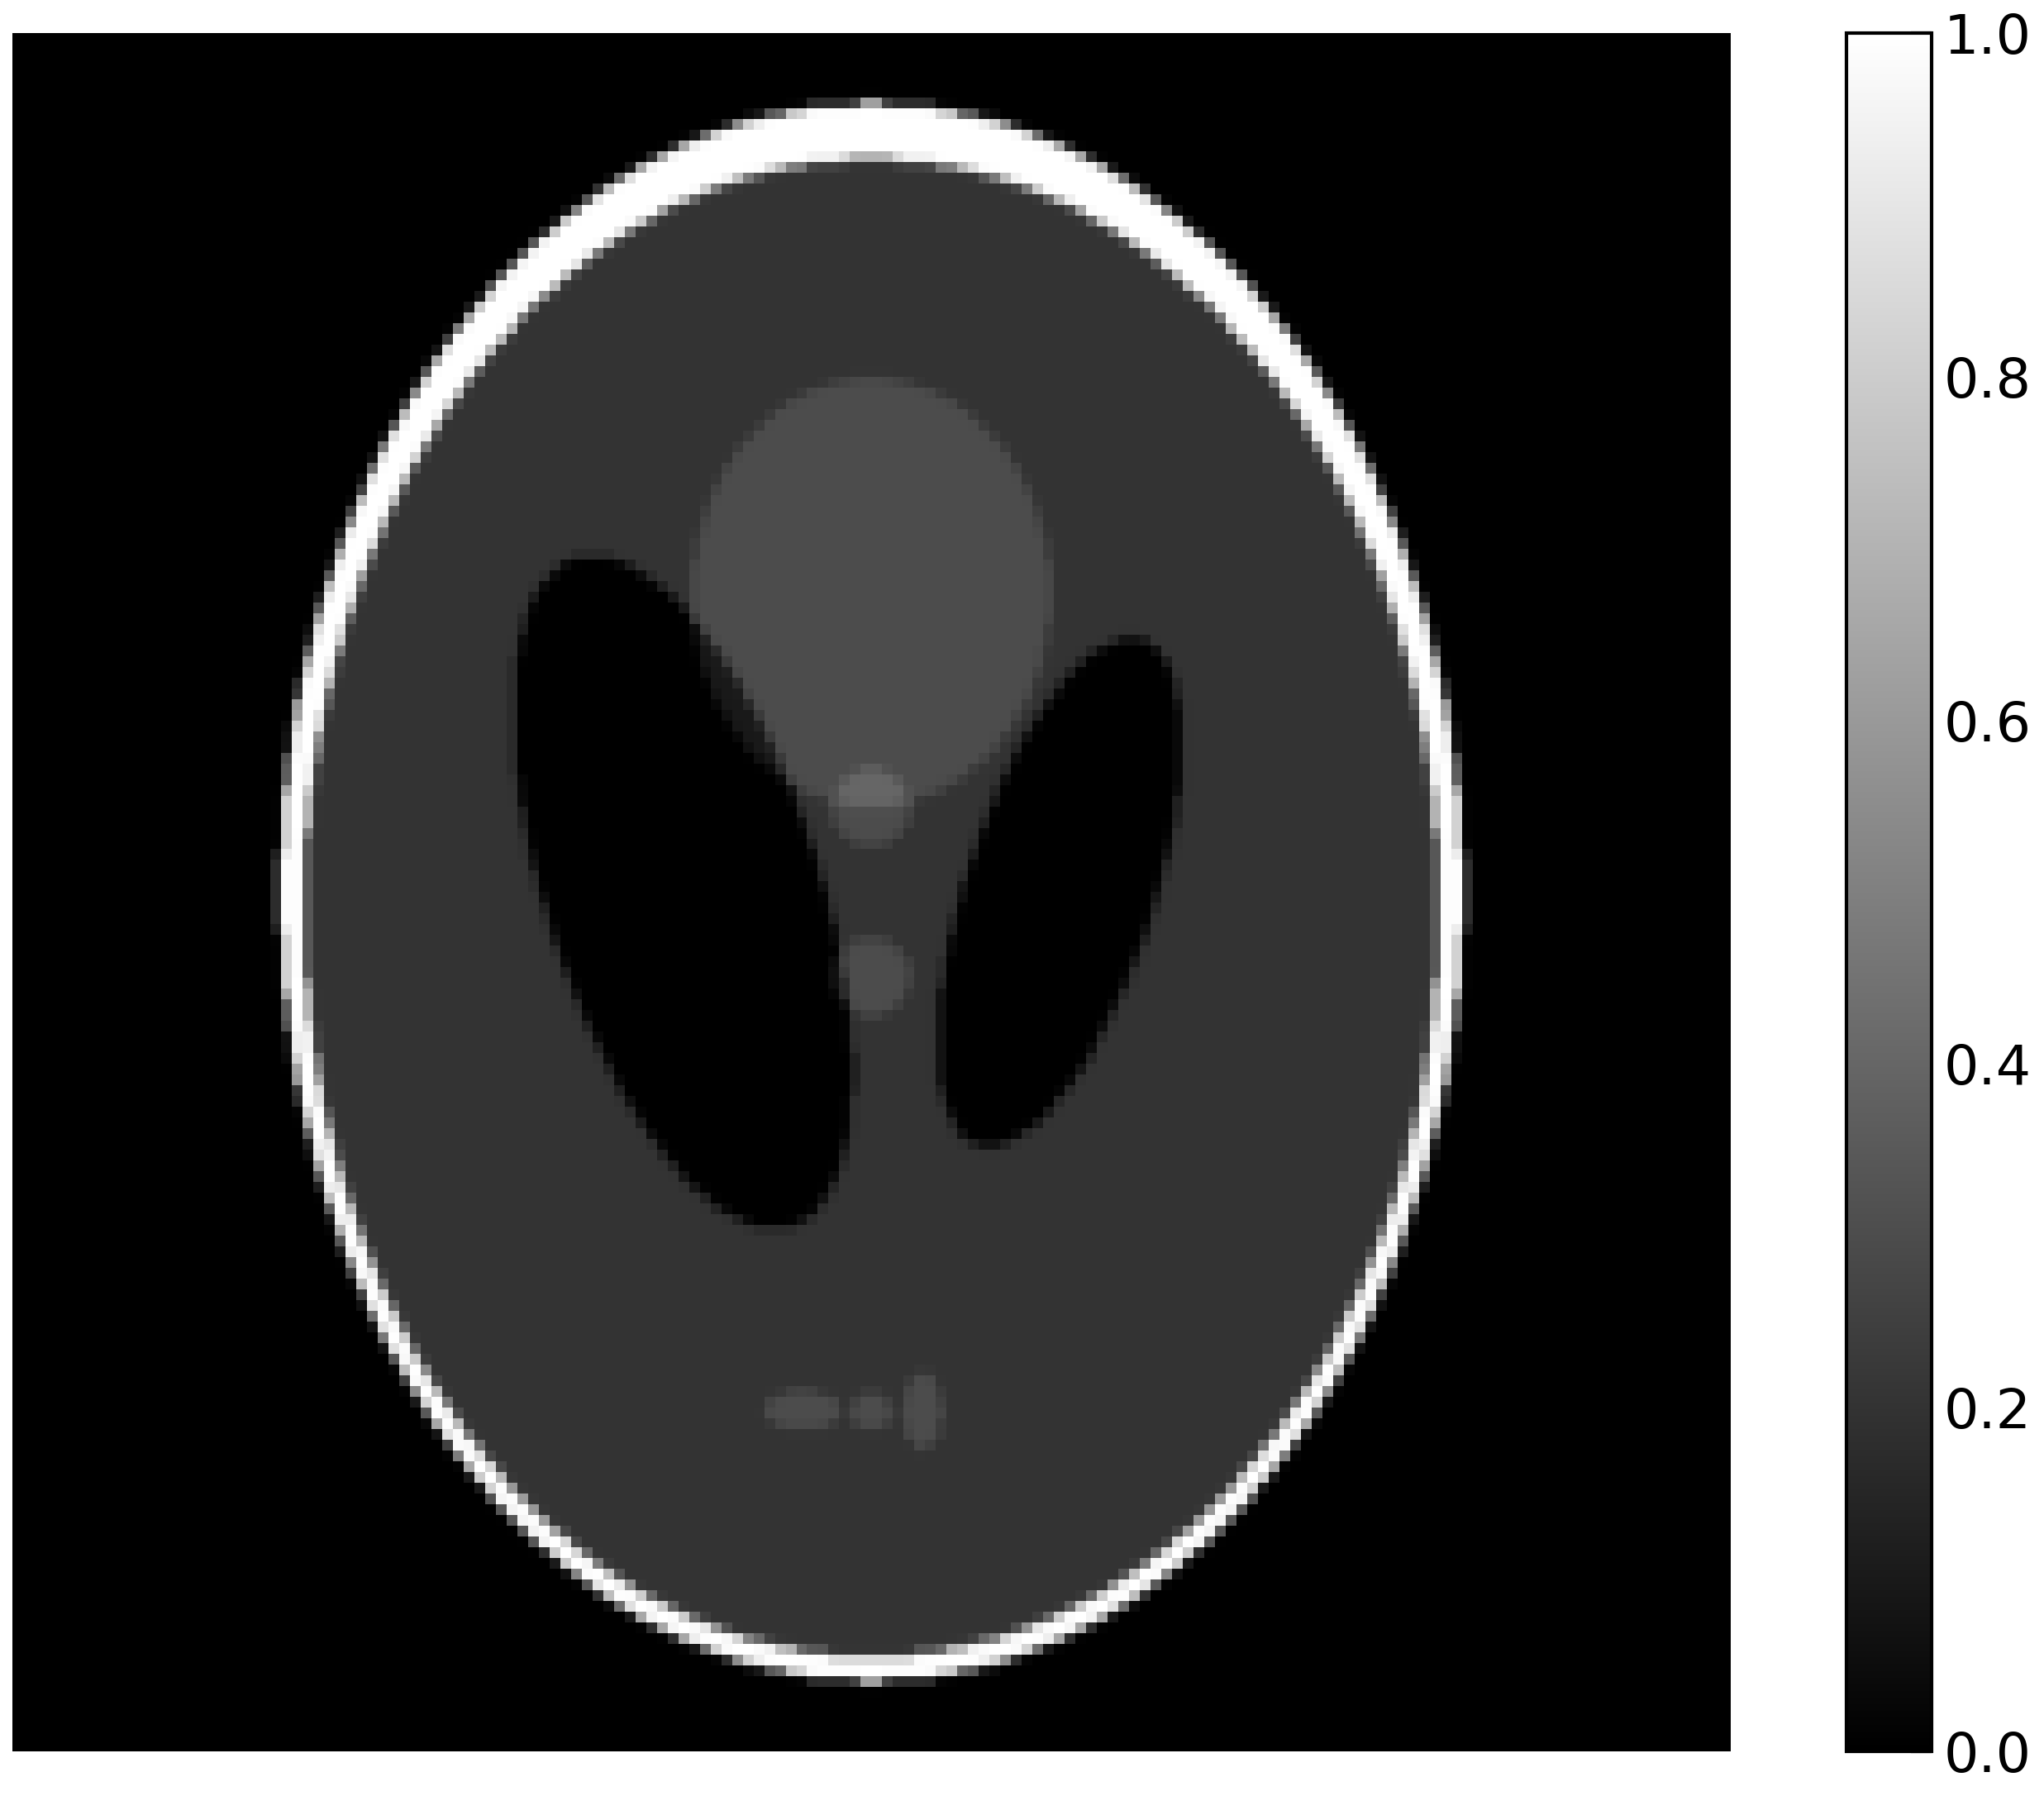
\includegraphics[width=0.24\textwidth]{images/ej_1/fantoma.png}\label{fig:fantoma_ej1}}
    \hfill
    \subfloat[]{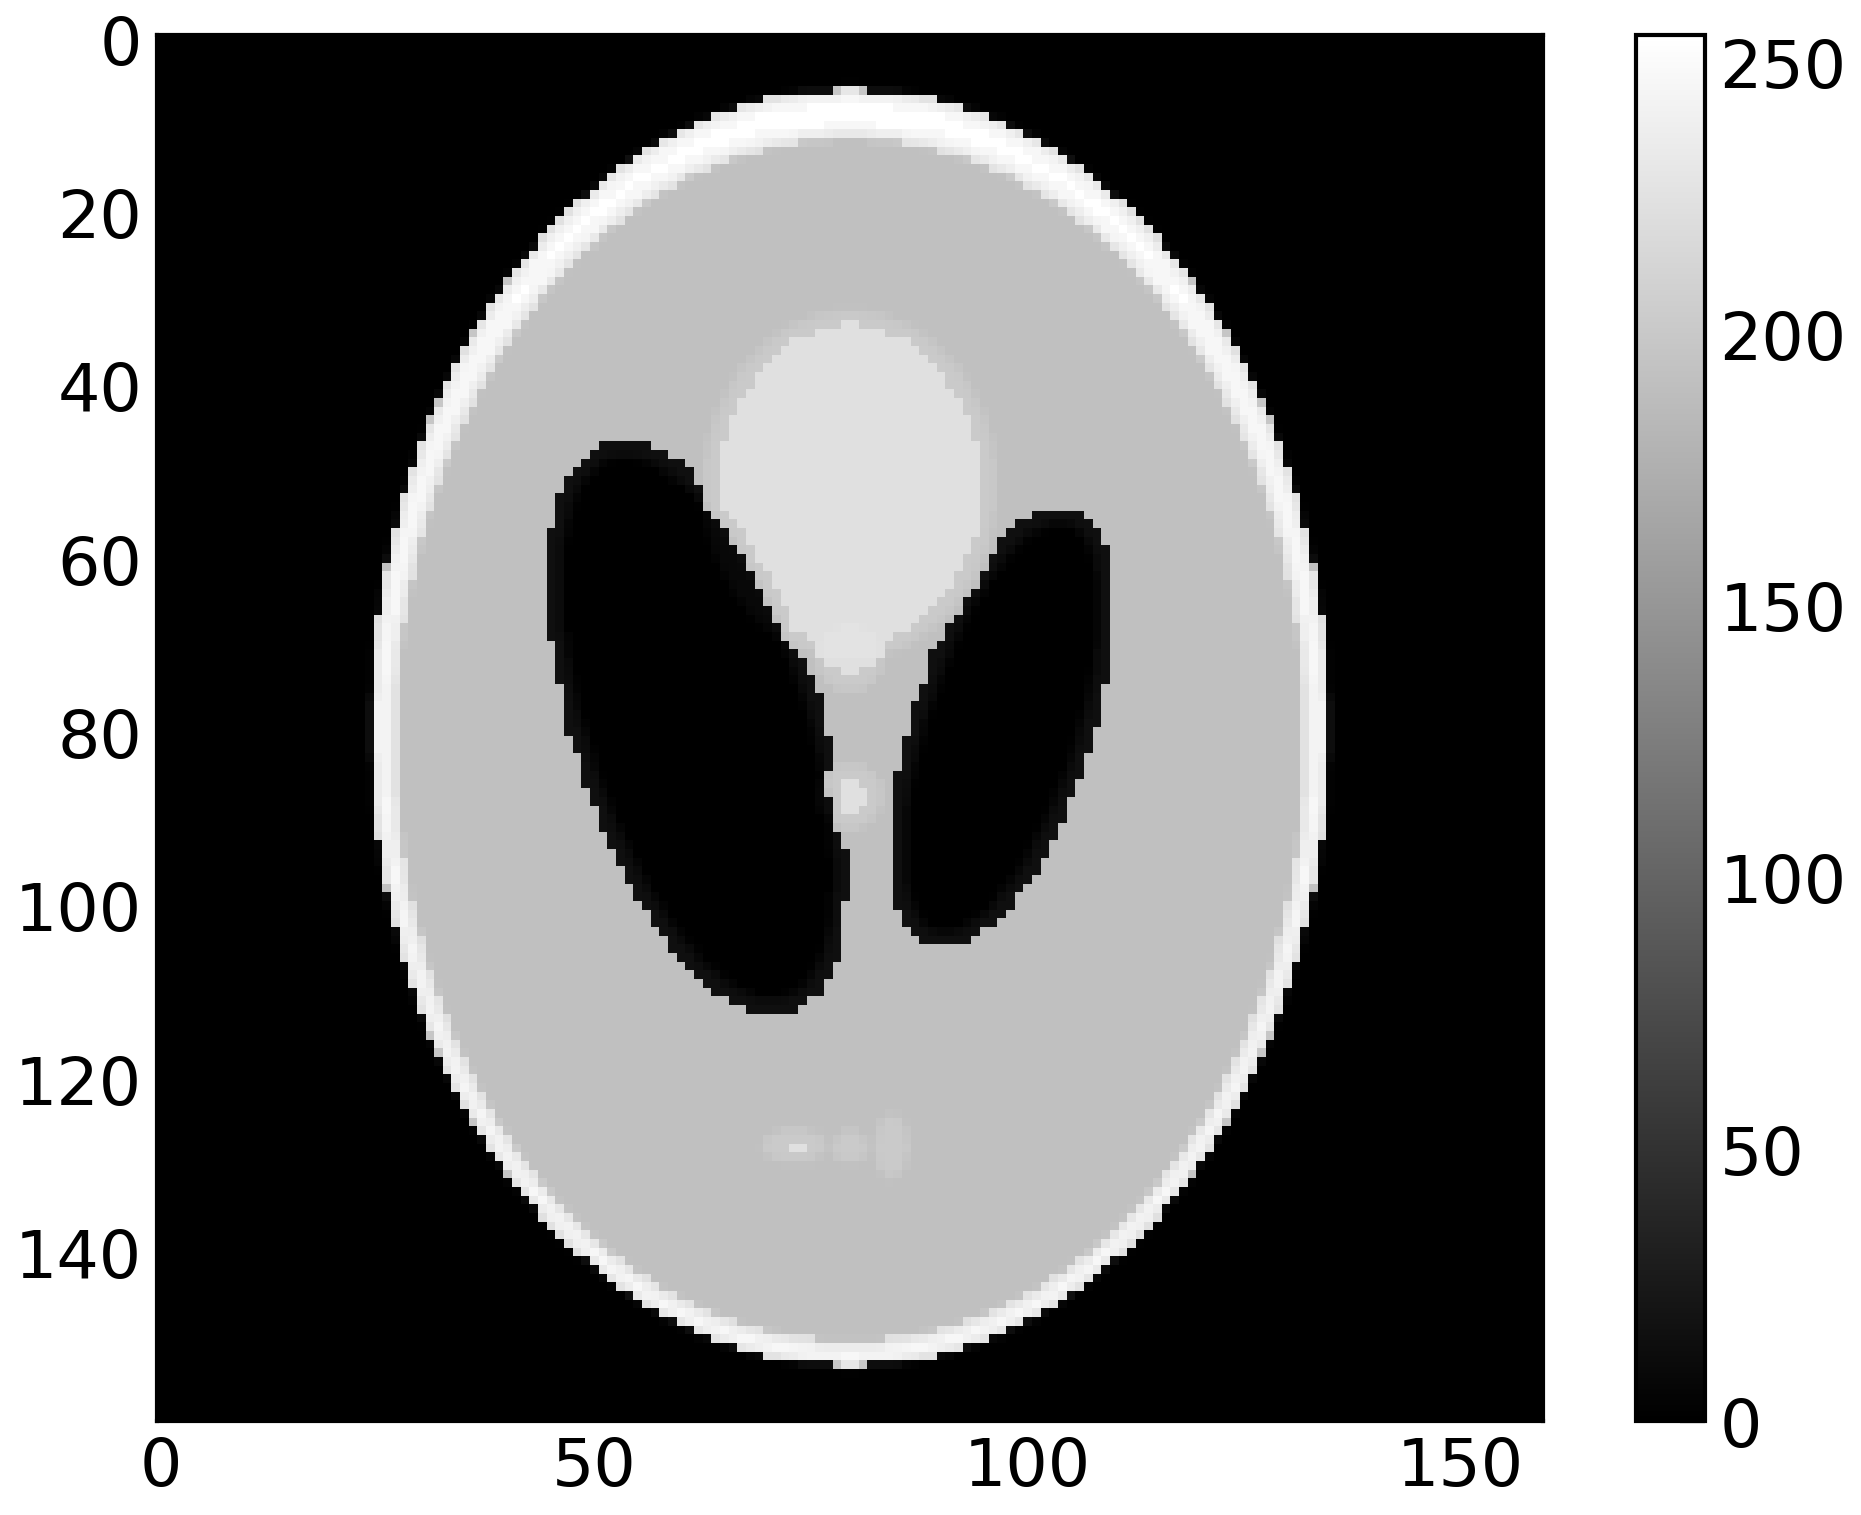
\includegraphics[width=0.24\textwidth]{images/ej_1/fantoma_eq.png}\label{fig:fantoma_eq}}
    \hfill
    \caption{(a) Fantoma \textit{Shepp-Logan} original. (b) Fantoma ecualizado. Ambas imágenes son de tamaño predeterminado: $160 \times 160$ píxeles.}
    \label{fig:figuras_ej_1}
  \end{figure}

% --------------- EJ 2 ---------------------
\subsection*{Ejercicio 2}
Para obtener las proyecciones del fantoma del ejercicio anterior se utilizó la función \href{https://scikit-image.org/docs/stable/api/skimage.transform.html#skimage.transform.radon}{\texttt{radon}} del modulo \href{https://scikit-image.org/docs/stable/api/skimage.transform.html#}{\texttt{transform}} de la librería \texttt{skimage}. Se obtuvieron las proyecciones para 120 ángulos $\theta$ equiespaciados entre 0 y 180 grados. El sinograma resultante se muestra en la Figura \ref{fig:sinograma_ej_2}.

\begin{figure} [htbp]
    \centering
    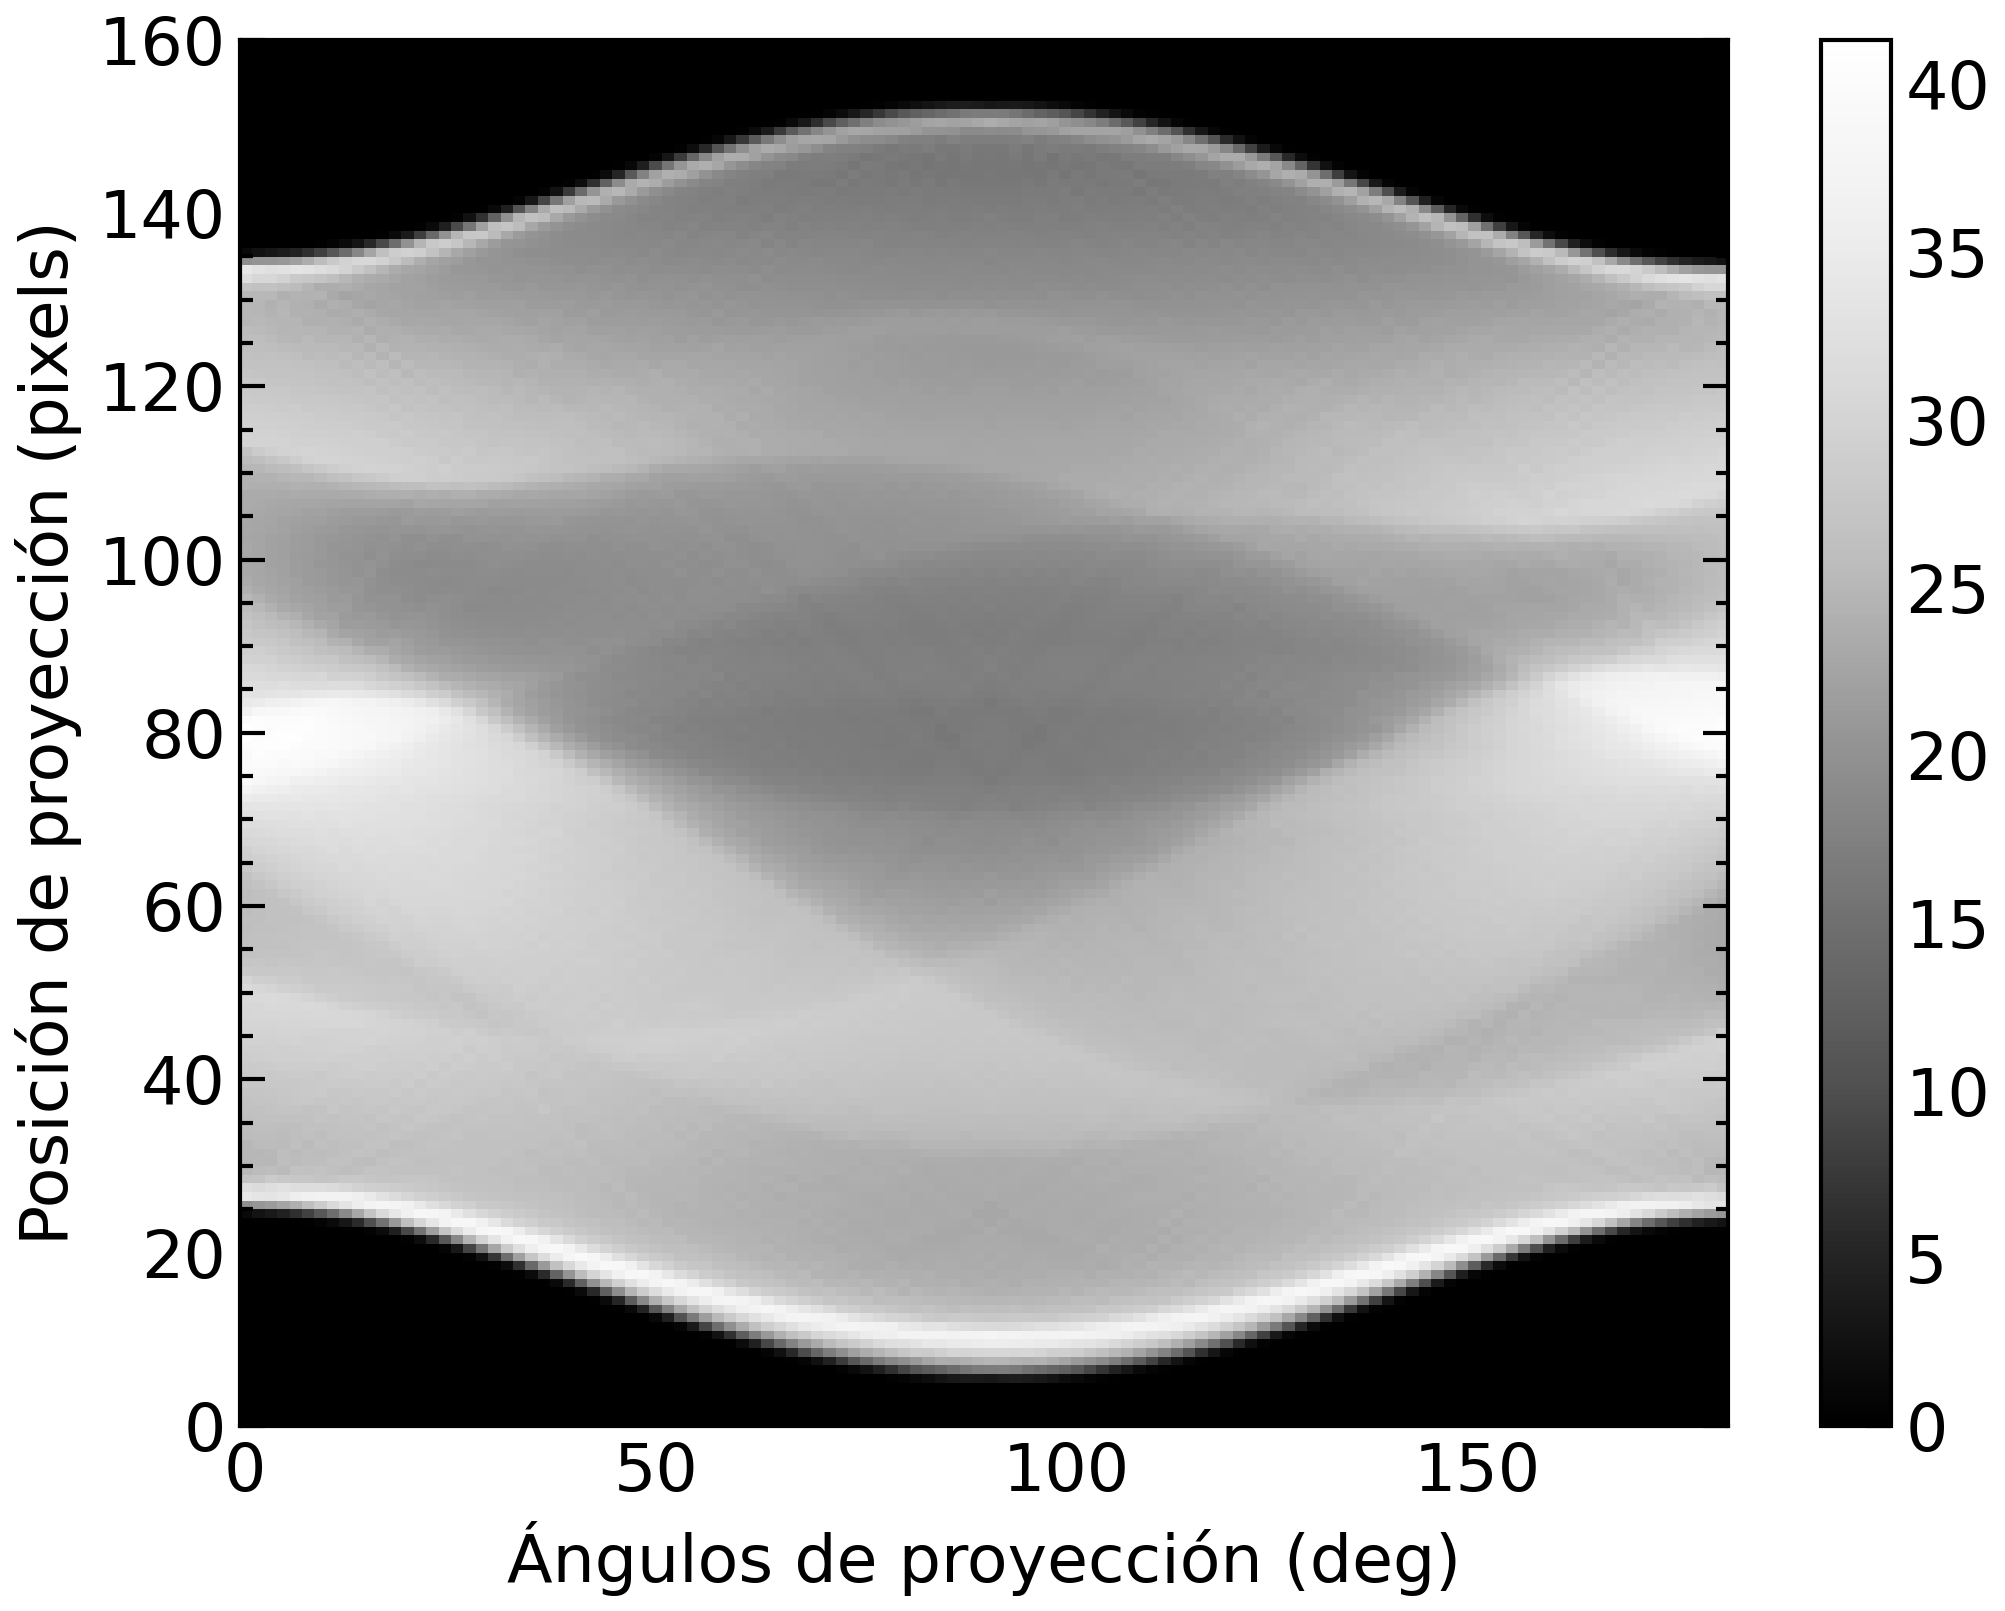
\includegraphics[width=0.5\textwidth]{images/ej_2/sinogram.png}
    \caption{Sinograma del fantoma de \textit{Shepp-Logan} con 120 ángulos $\theta$ equiespaciados entre 0 y 180 grados, suponiendo que el detector tiene un ancho de 160 píxeles.}
    \label{fig:sinograma_ej_2}
\end{figure}

% --------------- EJ 3 ---------------------
\subsection*{Ejercicio 3}
Se utilizó el algoritmo de \textit{Retroproyección Filtrada} para reconstruir la imagen del fantoma a partir del sinograma obtenido en el ejercicio anterior. Para ello, se utilizó la función \href{https://scikit-image.org/docs/stable/api/skimage.transform.html#skimage.transform.iradon}{\texttt{iradon}} del modulo \texttt{transform} de la librería \texttt{skimage}. Para la Reconstrucción de la imagen es posible utilizar diferentes tipos de filtros, como pueden ser: \textit{Ramp}, \textit{Shepp-Logan}, \textit{Cosine}, \textit{Hamming}, \textit{Hann}, entre otros. En la Figura \ref{fig:filtros} se muestra el efecto de cada uno de estos filtros en función de la frecuencia.

\begin{figure} [htbp]
    \centering
    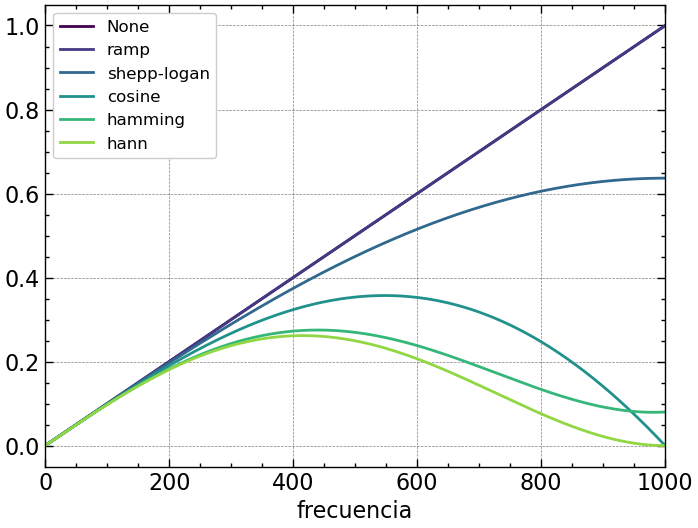
\includegraphics[width=0.45\textwidth]{images/ej_3/fourier_filters.png}
    \caption{filtros normalizados en el dominio de la frecuencia.}
    \label{fig:filtros}
\end{figure}

Los filtros en la Figura \ref{fig:filtros} tienen características distintas, destacando en qué frecuencias enfatizan. El filtro \textit{Ramp} es uno de los más básico, sin distorsiones notables en la imagen, pero no atenúa significativamente las frecuencias altas. En cambio, los otros filtros son más agresivos al reducir las altas frecuencias.

Se aplicó cada filtro, y se calculó el error cuadrático medio (ECM) entre la imagen original y la reconstruida. La Tabla \ref{tab:error} se muestran los resultados, mientras que en la Figura \ref{fig:figuras_ej_3} se visualiza la imagen reconstruida y la diferencia entre esta y la imagen original para el filtro \textit{Ramp}.

\begin{table}[H]
    \centering
    \begin{tabular}{|c|c|}
    \hline
    \textbf{Filtro} & \textbf{Error} \\ \hline
    \textit{Ramp}             & 0.0286           \\ \hline
    \textit{Shepp-Logan}             & 0.033           \\ \hline
    \textit{Cosine}             & 0.0421           \\ \hline
    \textit{Hamming}             & 0.0496           \\ \hline
    \textit{Hann}             & 0.0516           \\ \hline
    \end{tabular}
    \caption{valores de error cuadrático medio (ECM) para cada filtro al realizar el algoritmo de retroproyección filtrada.}
    \label{tab:error}
  \end{table}

  \begin{figure}[H]
    \centering
    \subfloat[]{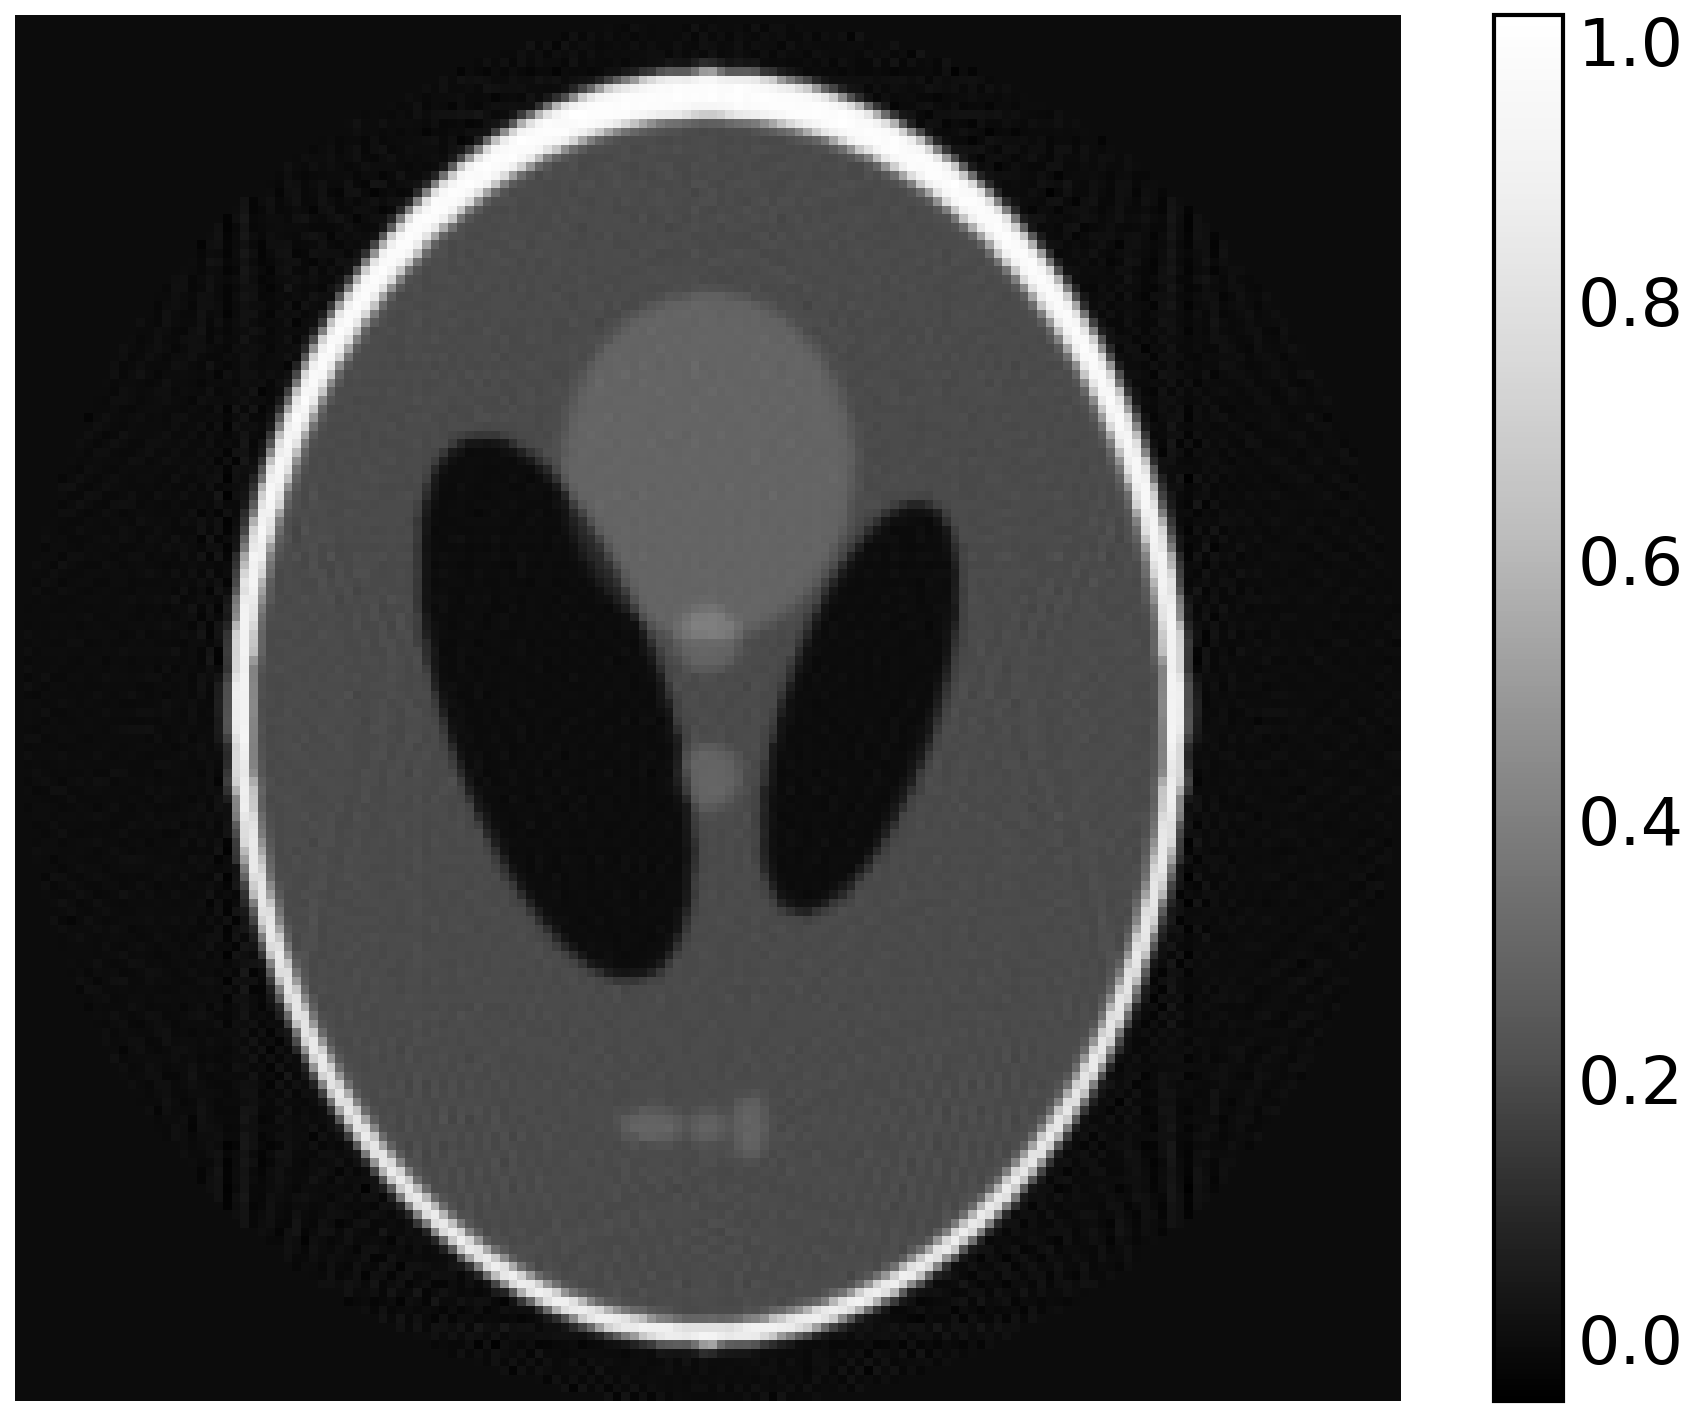
\includegraphics[width=0.24\textwidth]{images/ej_3/reconstruction_fbp.png}\label{fig:fbp_ej_3}}
    \hfill
    \subfloat[]{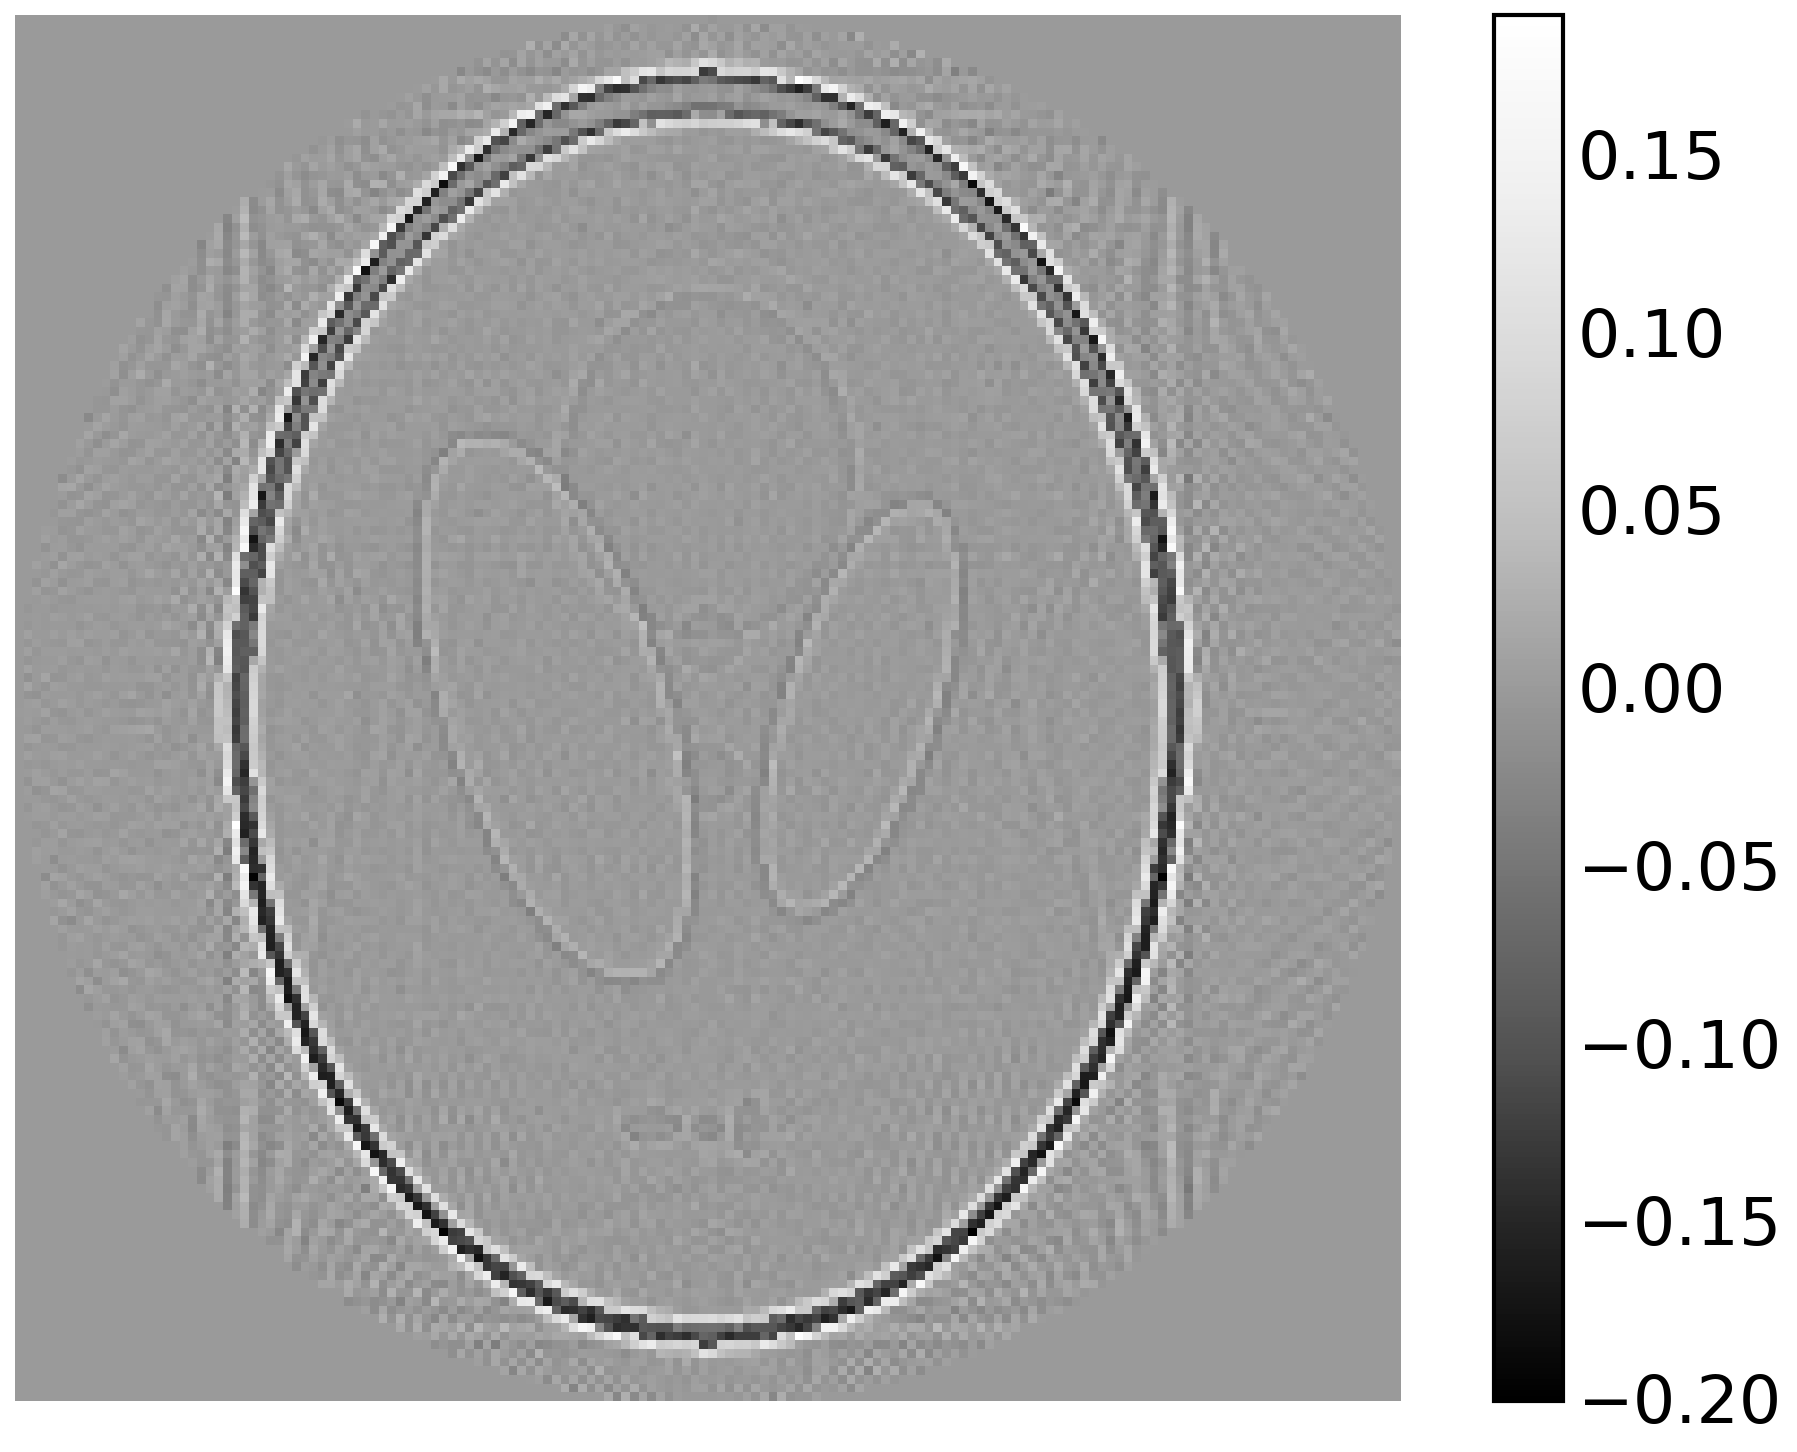
\includegraphics[width=0.24\textwidth]{images/ej_3/reconstruction_error.png}\label{fig:fbp_error_ej_3}}
    \hfill
    \caption{(a) fantoma \textit{Shepp-Logan} reconstruido con el algoritmo de retroproyección filtrada. (b) Diferencia entre la imagen reconstruida y la original.}
    \label{fig:figuras_ej_3}
  \end{figure}

% --------------- EJ 4 ---------------------
\subsection*{Ejercicio 4}
Se estudió el error que se comete en la Reconstrucción de la imagen en función de los parámetros de adquisición, como el número de detectores $N_d$ y los parámetros de reconstrucción, como el número de ángulos $N_\theta$. Para ello, inicialmente se fijó el número de ángulos en 120, y se varió el número de detectores $N_D$ entre 80 y 1200. Los resultados se muestran en la Figura \ref{fig:error_escalas}.

\begin{figure} [htbp]
    \centering
    \includegraphics*[width=0.5\textwidth]{./images/ej_4/scale_error_2.png}
    \caption{Error cuadrático medio (ECM) en función del número de detectores $N_D$ para $N_\theta = 120$.}
    \label{fig:error_escalas}
\end{figure}


En la Figura \ref{fig:error_escalas} se observa que para $N_D$ pequeños ($N_D \lesssim 500$), el filtro \textit{Ramp} produce un menor error. Sin embargo, cuando $N_D \approx 500$, todos los filtros tienen un error similar. A medida que $N_D$ aumenta, el orden de los filtros con menor error se invierte, siendo el filtro \textit{Ramp} el que produce un mayor error.

Un análisis similar se realizó variando el número de ángulos entre 10 y 200, manteniendo fijo el número de detectores $N_D = 160$. Los resultados se muestran en la Figura \ref{fig:error_angulos}.

\begin{figure} [htbp]
    \centering
    \includegraphics*[width=0.5\textwidth]{./images/ej_4/angle_error_2.png}
    \caption{Error cuadrático medio (ECM) en función del número de ángulos $N_\theta$ para $N_D = 160$.}
    \label{fig:error_angulos}
\end{figure}

En la Figura \ref{fig:error_angulos} se observa que para un número pequeño de ángulos ($N_\theta \lesssim 40$), el filtro \textit{Hann} produce un error ligeramente menor. Sin embargo, a medida que $\theta$ aumenta ($N_\theta \gtrsim 40$), el filtro \textit{Ramp} produce un error menor que los otros filtros. A partir de $N_\theta \approx 75$, la diferencia entre el error de los filtros a medida que $N_\theta$ aumenta constante.

% --------------- EJ 5 ---------------------
\subsection*{Ejercicio 5}
Para evaluar la respuesta del algoritmo de retroproyección filtrada ante la presencia de ruido, se introdujo ruido gaussiano en el sinograma del fantoma. Se empleó la función \href{https://numpy.org/doc/stable/reference/random/generated/numpy.random.normal.html}{\texttt{normal}} del módulo \href{https://numpy.org/doc/stable/reference/random/index.html}{\texttt{numpy.random}}, con una media de 0 y una desviación estándar de 1. Los valores generados fueron multiplicados por un factor \textit{level} de 2 para controlar el nivel de ruido. En la Figura \ref{fig:sinograma_ruido} se muestra el sinograma con ruido agregado.

\begin{figure} [htbp]
    \centering
    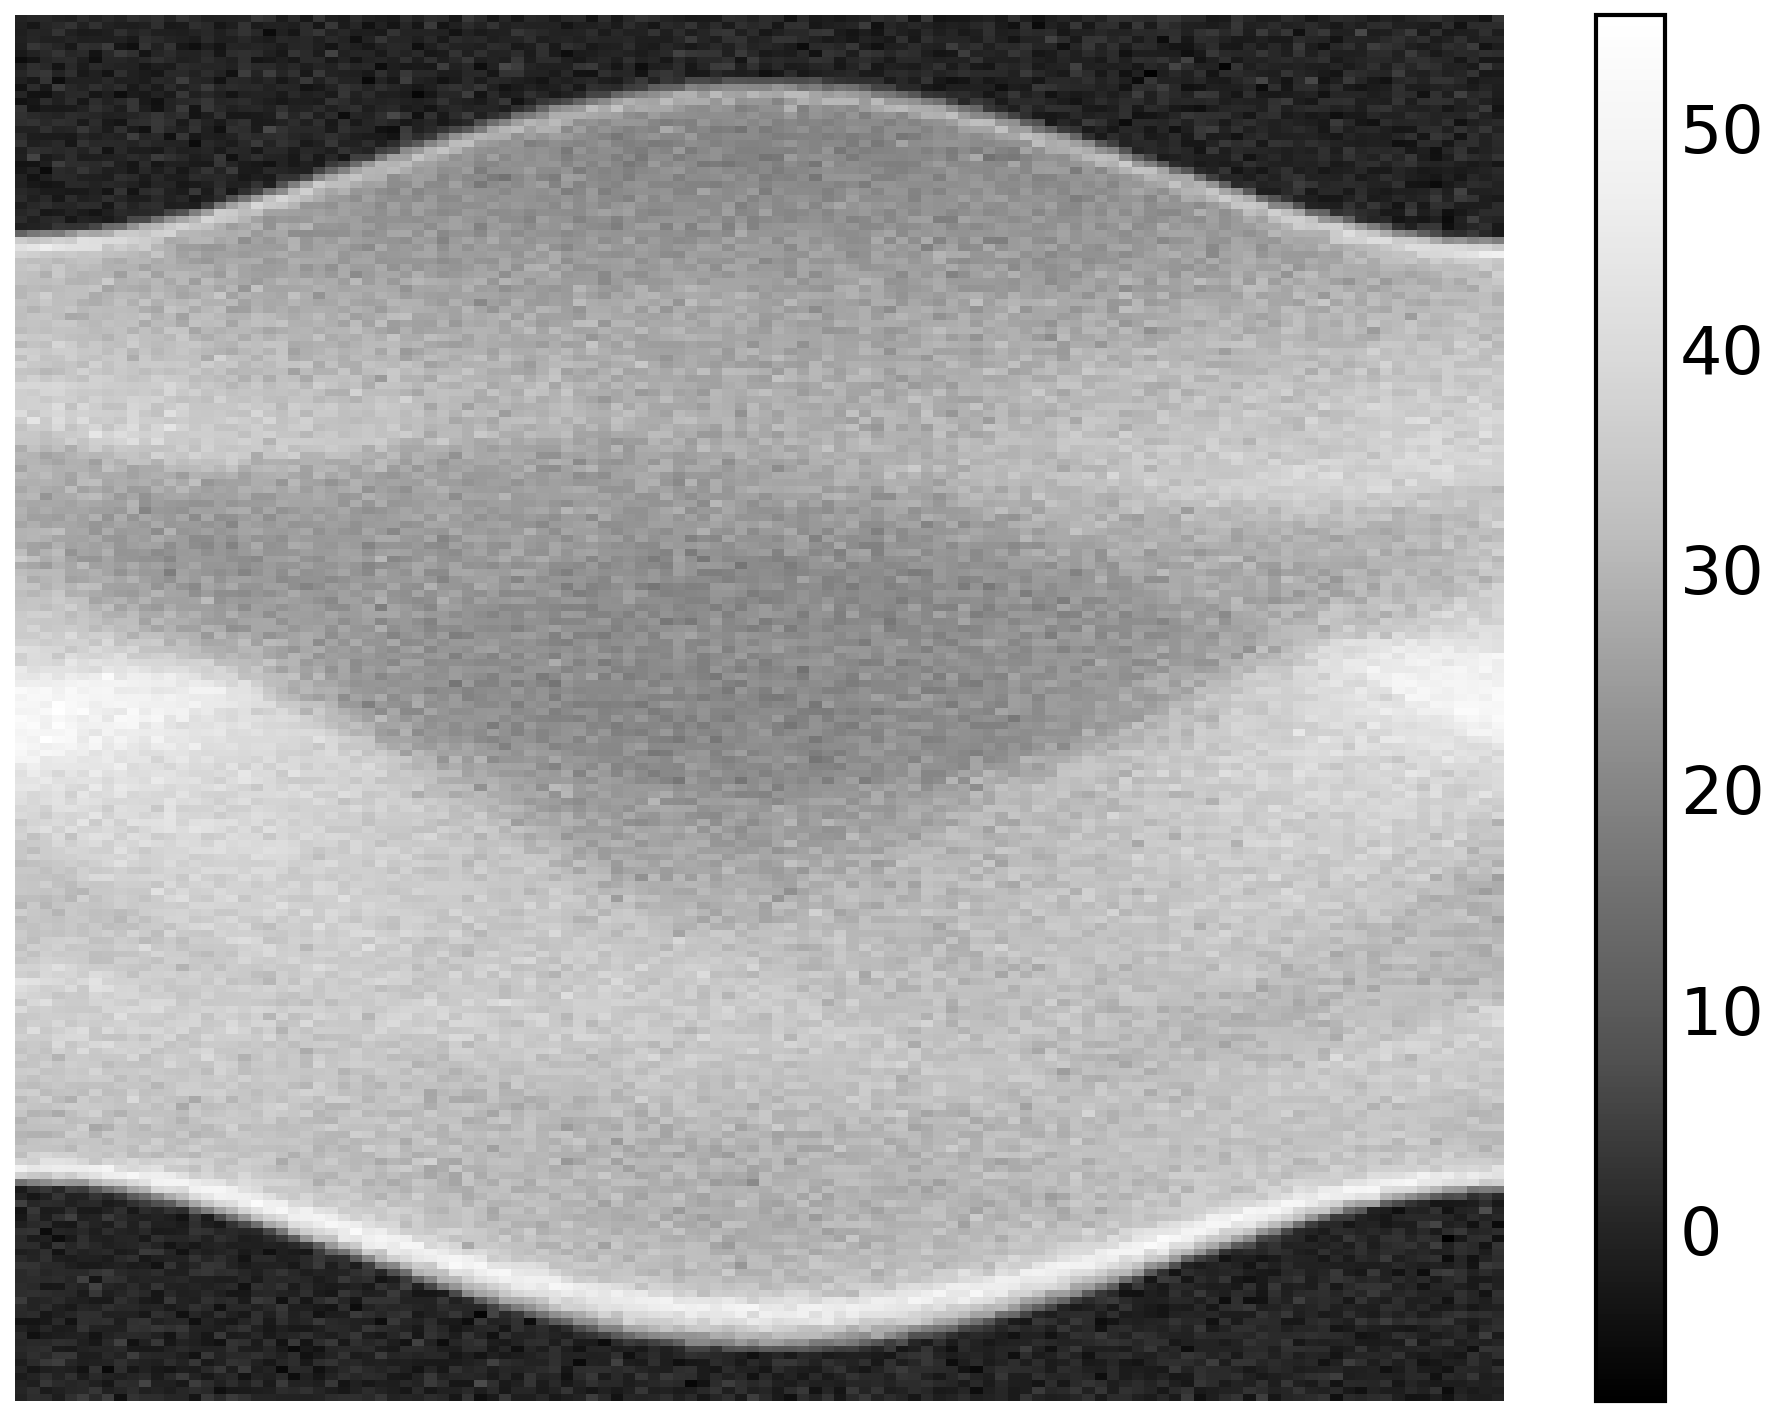
\includegraphics[width=0.5\textwidth]{images/ej_5/sinogram_noisy.png}
    \caption{sinograma del fantoma de \textit{Shepp-Logan} con ruido gaussiano agregado con un \textit{level} de 2.}
    \label{fig:sinograma_ruido}
\end{figure}

Se realizó un análisis similar al ejercicio 4, variando el número de detectores $N_D$ entre 80 y 1200, con $N_\theta$ fijo en 120, y luego modificando $N_\theta$ entre 10 y 200, manteniendo $N_D$ constante en 160. La diferencia radica en que, en este caso, la imagen retroproyectada se generó a partir del sinograma ruidoso. Los resultados se muestran en las Figuras \ref{fig:error_escalas_ruido} y \ref{fig:error_angulos_ruido}.

\begin{figure} [htbp]
    \centering
    \includegraphics*[width=0.5\textwidth]{./images/ej_5/scale_error_noisy.png}
    \caption{error cuadrático medio (ECM) en relación con el número de detectores $N_D$ para un caso con $N_\theta = 120$, donde se introdujo ruido mediante un factor \textit{level} igual a 2.}
    \label{fig:error_escalas_ruido}
\end{figure}

\begin{figure} [htbp]
    \centering
    \includegraphics*[width=0.5\textwidth]{./images/ej_5/angle_error_noisy.png}
    \caption{error cuadrático medio (ECM) en relación con el número de ángulos $N_\theta$ para un caso con $N_D = 160$, donde se incorporó ruido con un factor \textit{level} de 2.}
    \label{fig:error_angulos_ruido}
\end{figure}

En las Figuras \ref{fig:error_escalas_ruido} y \ref{fig:error_angulos_ruido} se observa que con el agregado de ruido, el filtro de tipo \textit{Hann} es el que produce un error menor. Por contrario, el filtro \textit{Ramp} es el que produce un mayor error, independientemente de la cantidad de detectores o ángulos. La razón de esto es que el filtro \textit{Ramp} reduce de manera menos efectiva las frecuencias altas. En consecuencia, el ruido presente en estas frecuencias no es suficientemente filtrado, lo que resulta en la aparición de artefactos en la imagen reconstruida.

En la figura \ref{fig:reconstruccion_ruido} se muestra la imagen reconstruida con diferentes filtros, para un caso con $N_D = 200$ y $N_\theta = 120$, donde se introdujo ruido mediante un factor \textit{level} igual a 2.

\begin{figure}[H]
    \centering
    \subfloat[]{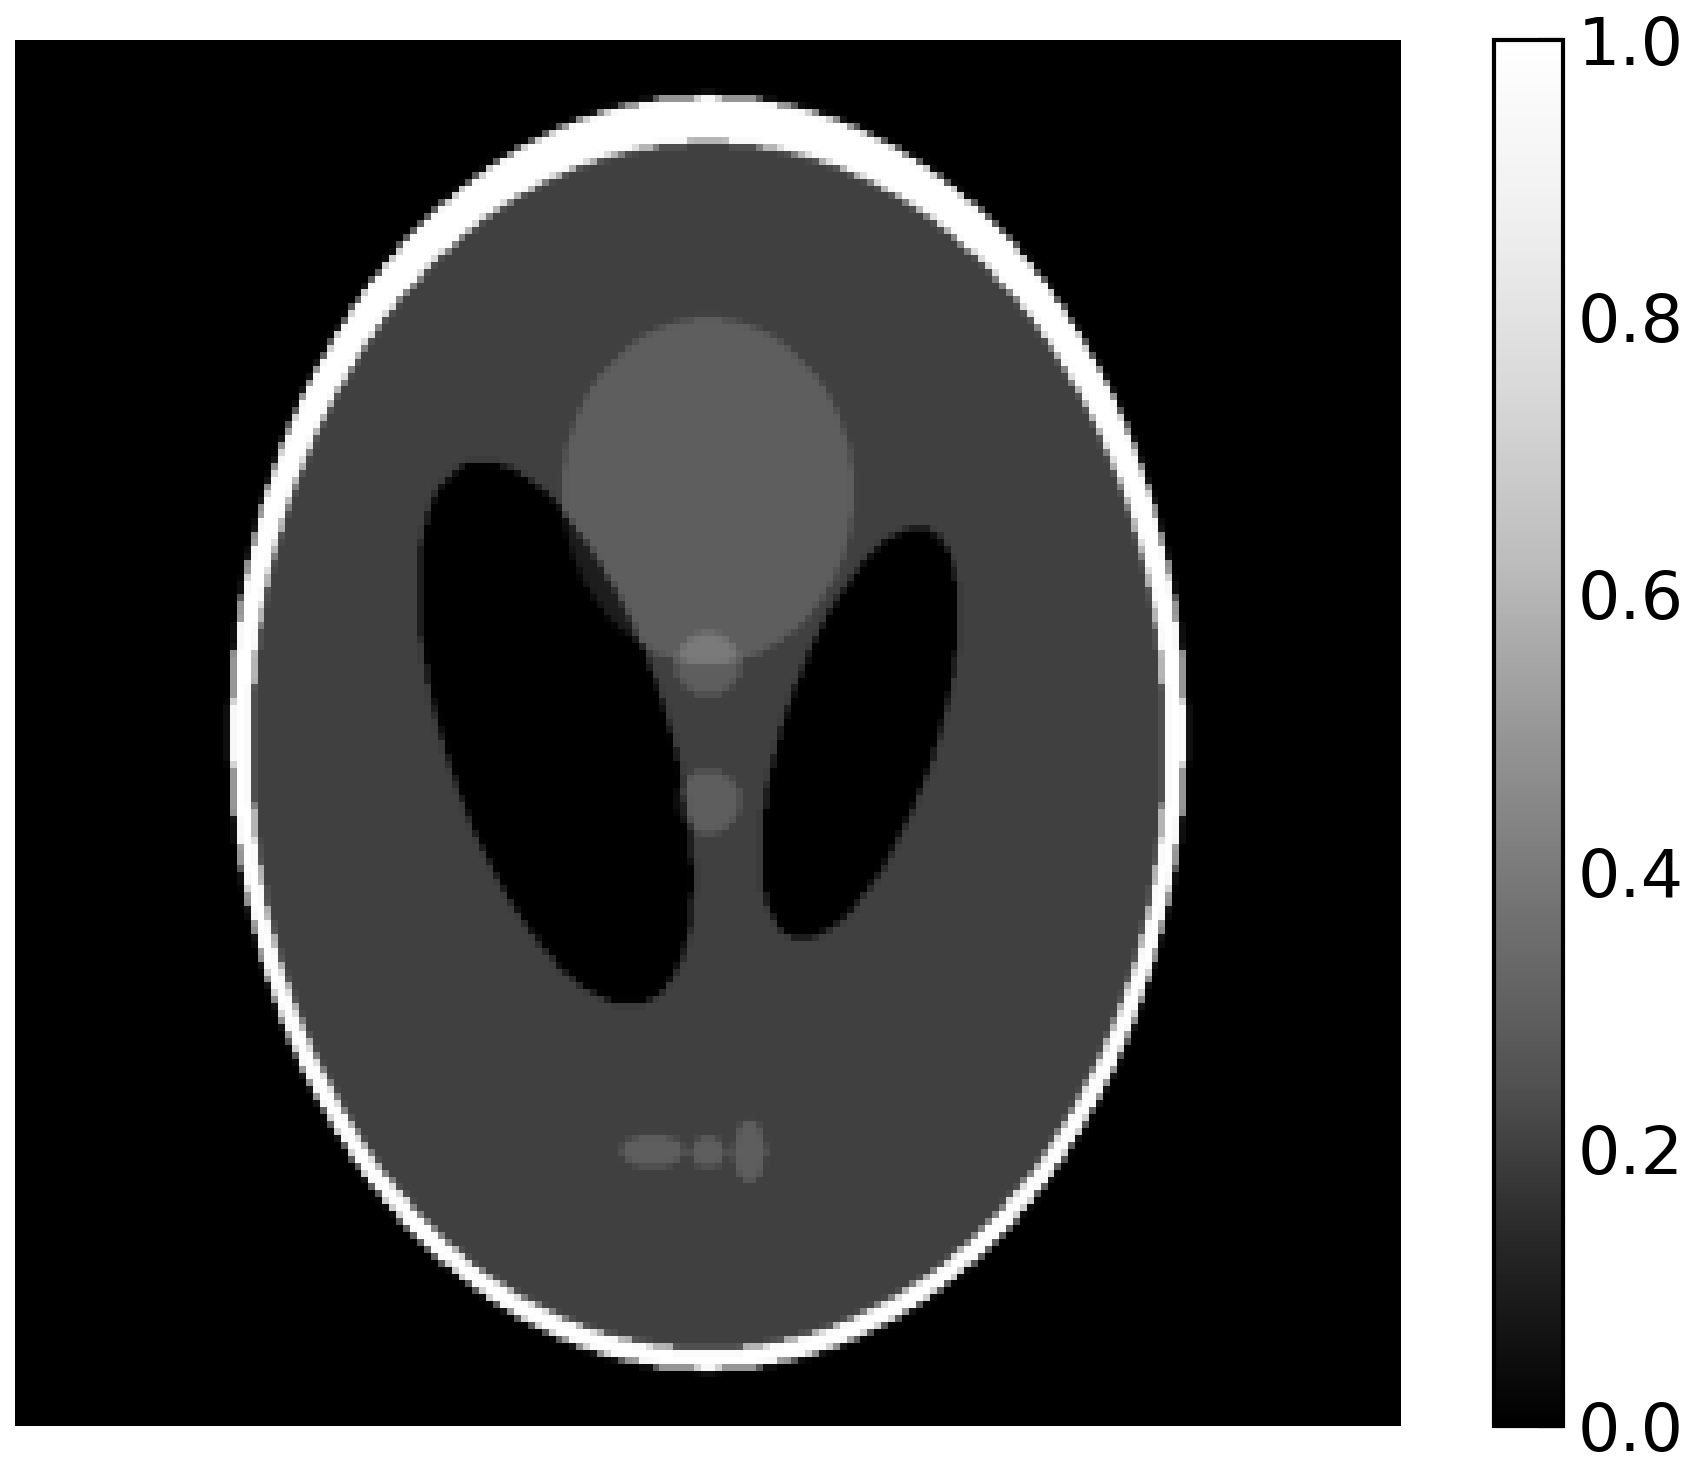
\includegraphics[width=0.24\textwidth]{images/ej_5/reconstruction_original.png}\label{fig:fbp_original_ej_5}}
    \hfill
    \subfloat[]{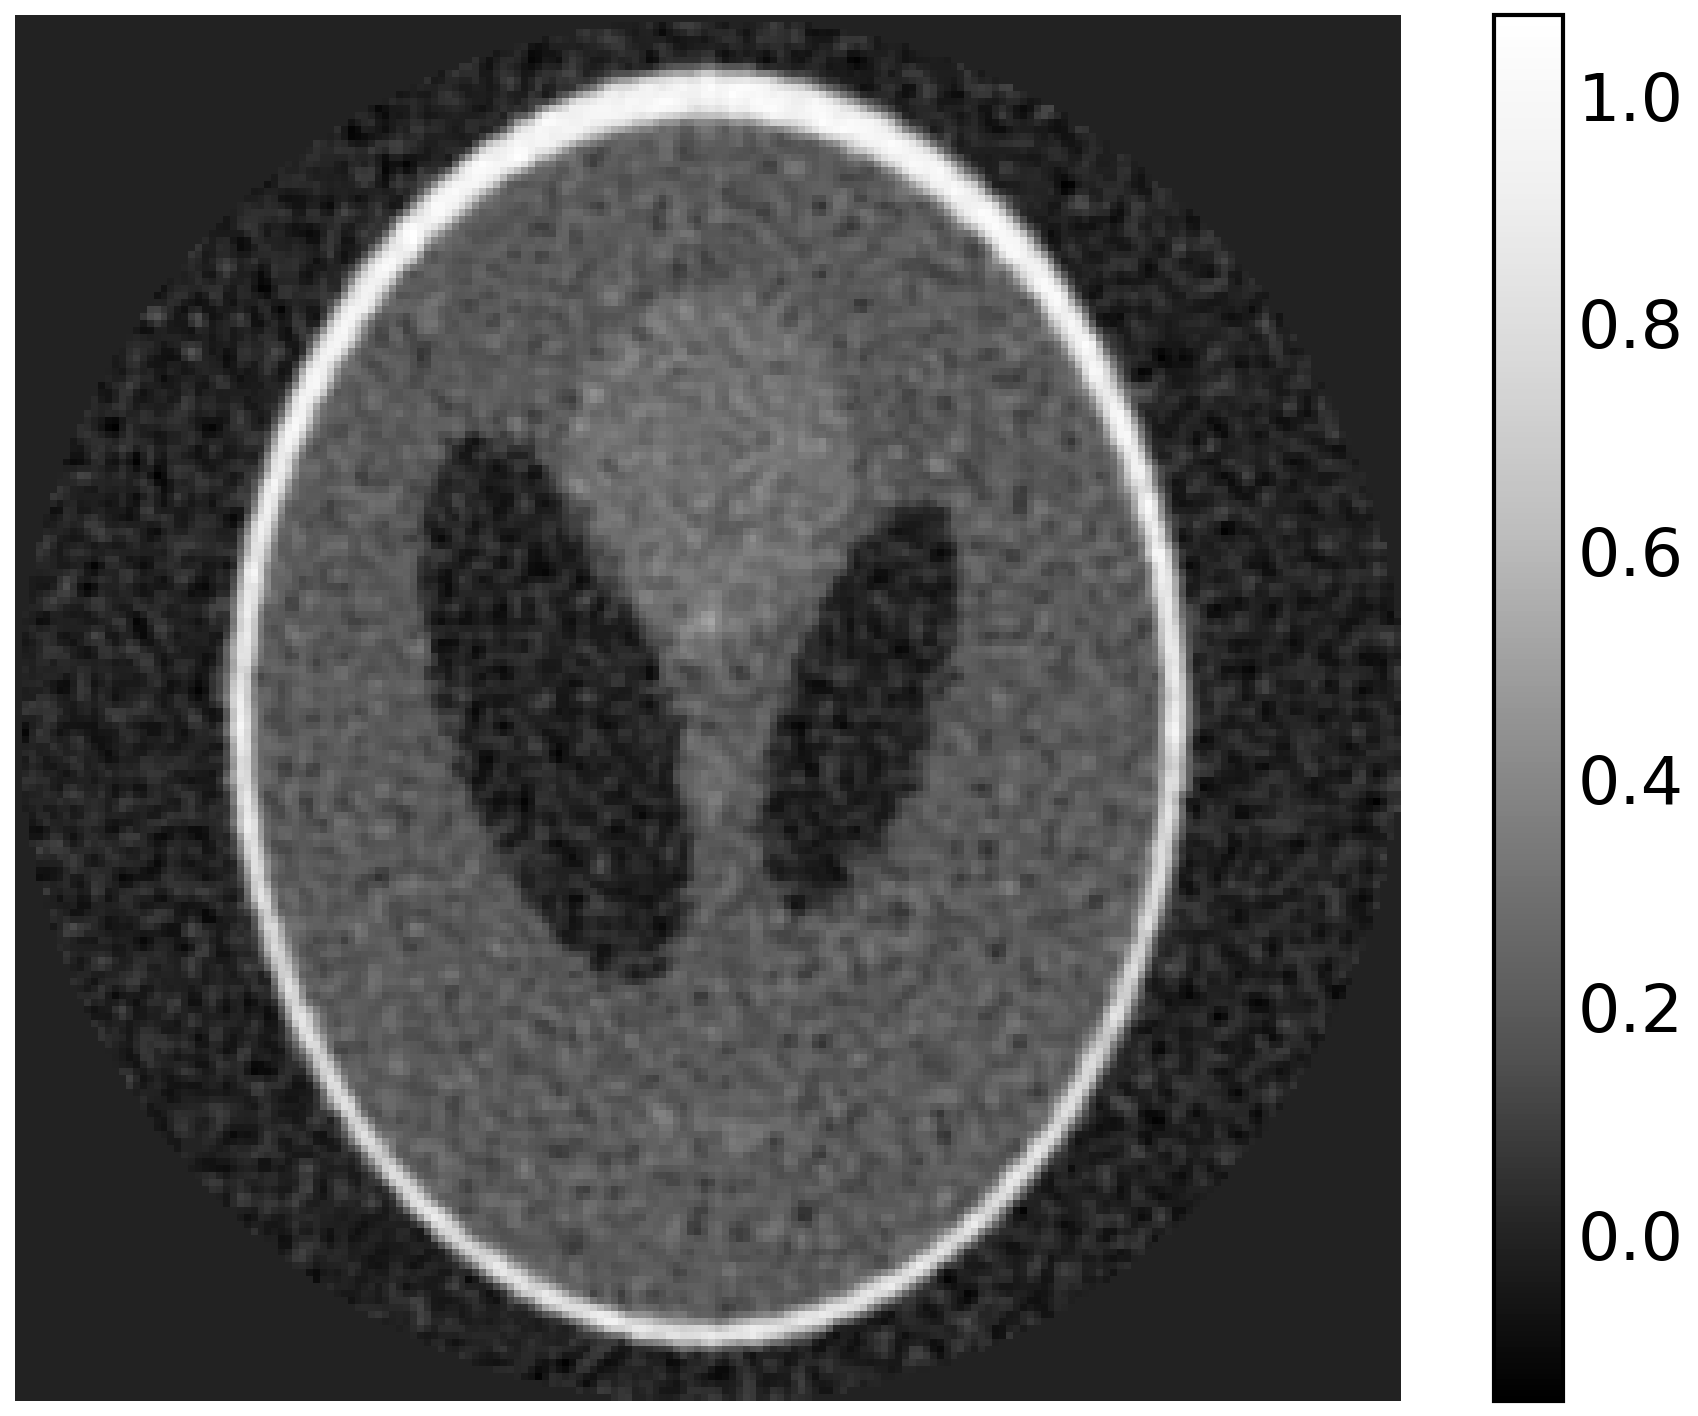
\includegraphics[width=0.24\textwidth]{images/ej_5/reconstruction_hann.png}\label{fig:fbp_hann_ej_5}}
    \hfill
    \subfloat[]{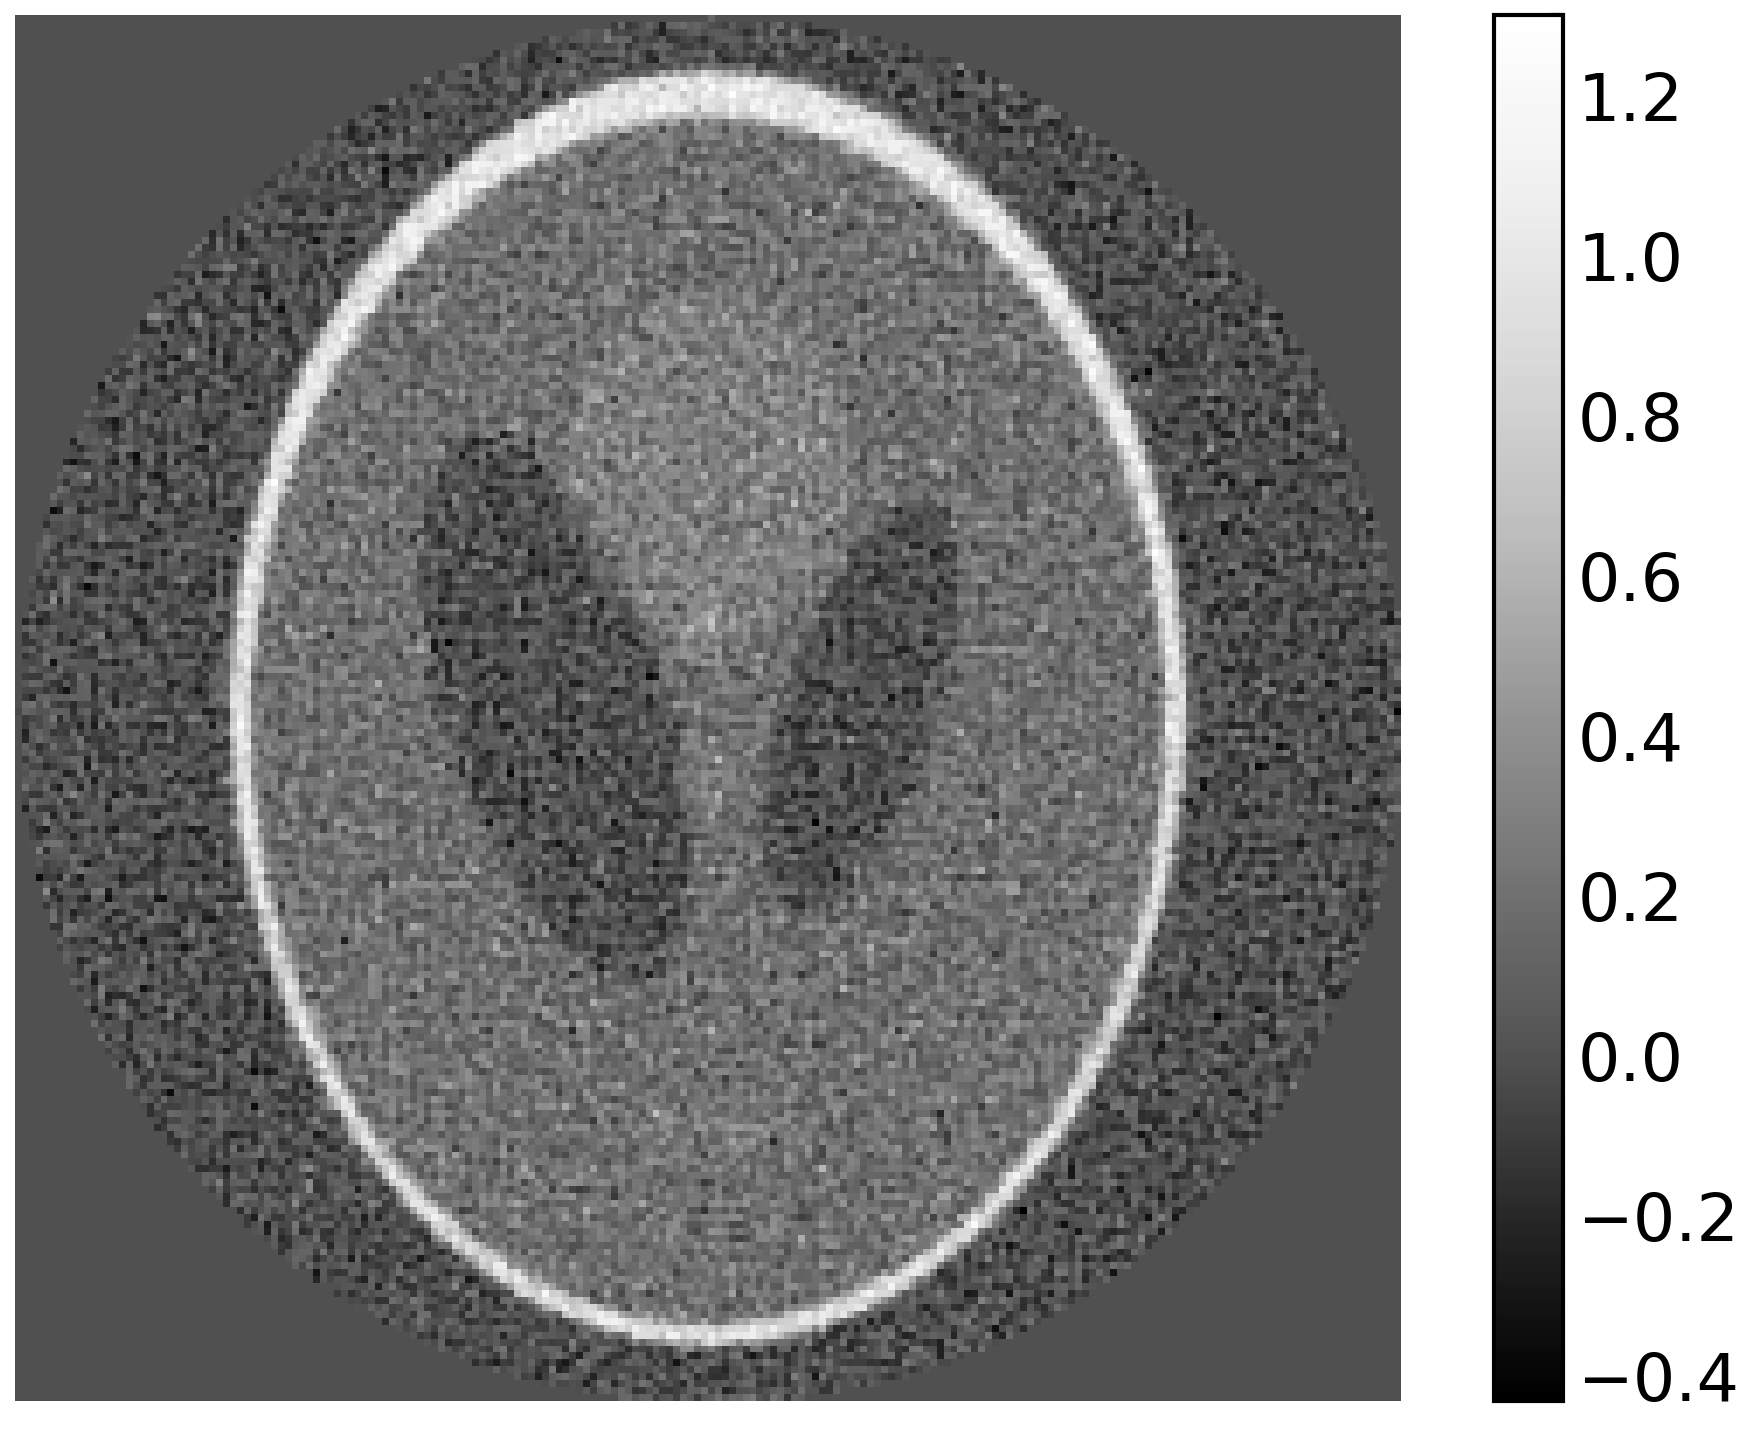
\includegraphics[width=0.24\textwidth]{images/ej_5/reconstruction_ramp.png}\label{fig:fbp_ramp_ej_5}}
    \hfill
    \subfloat[]{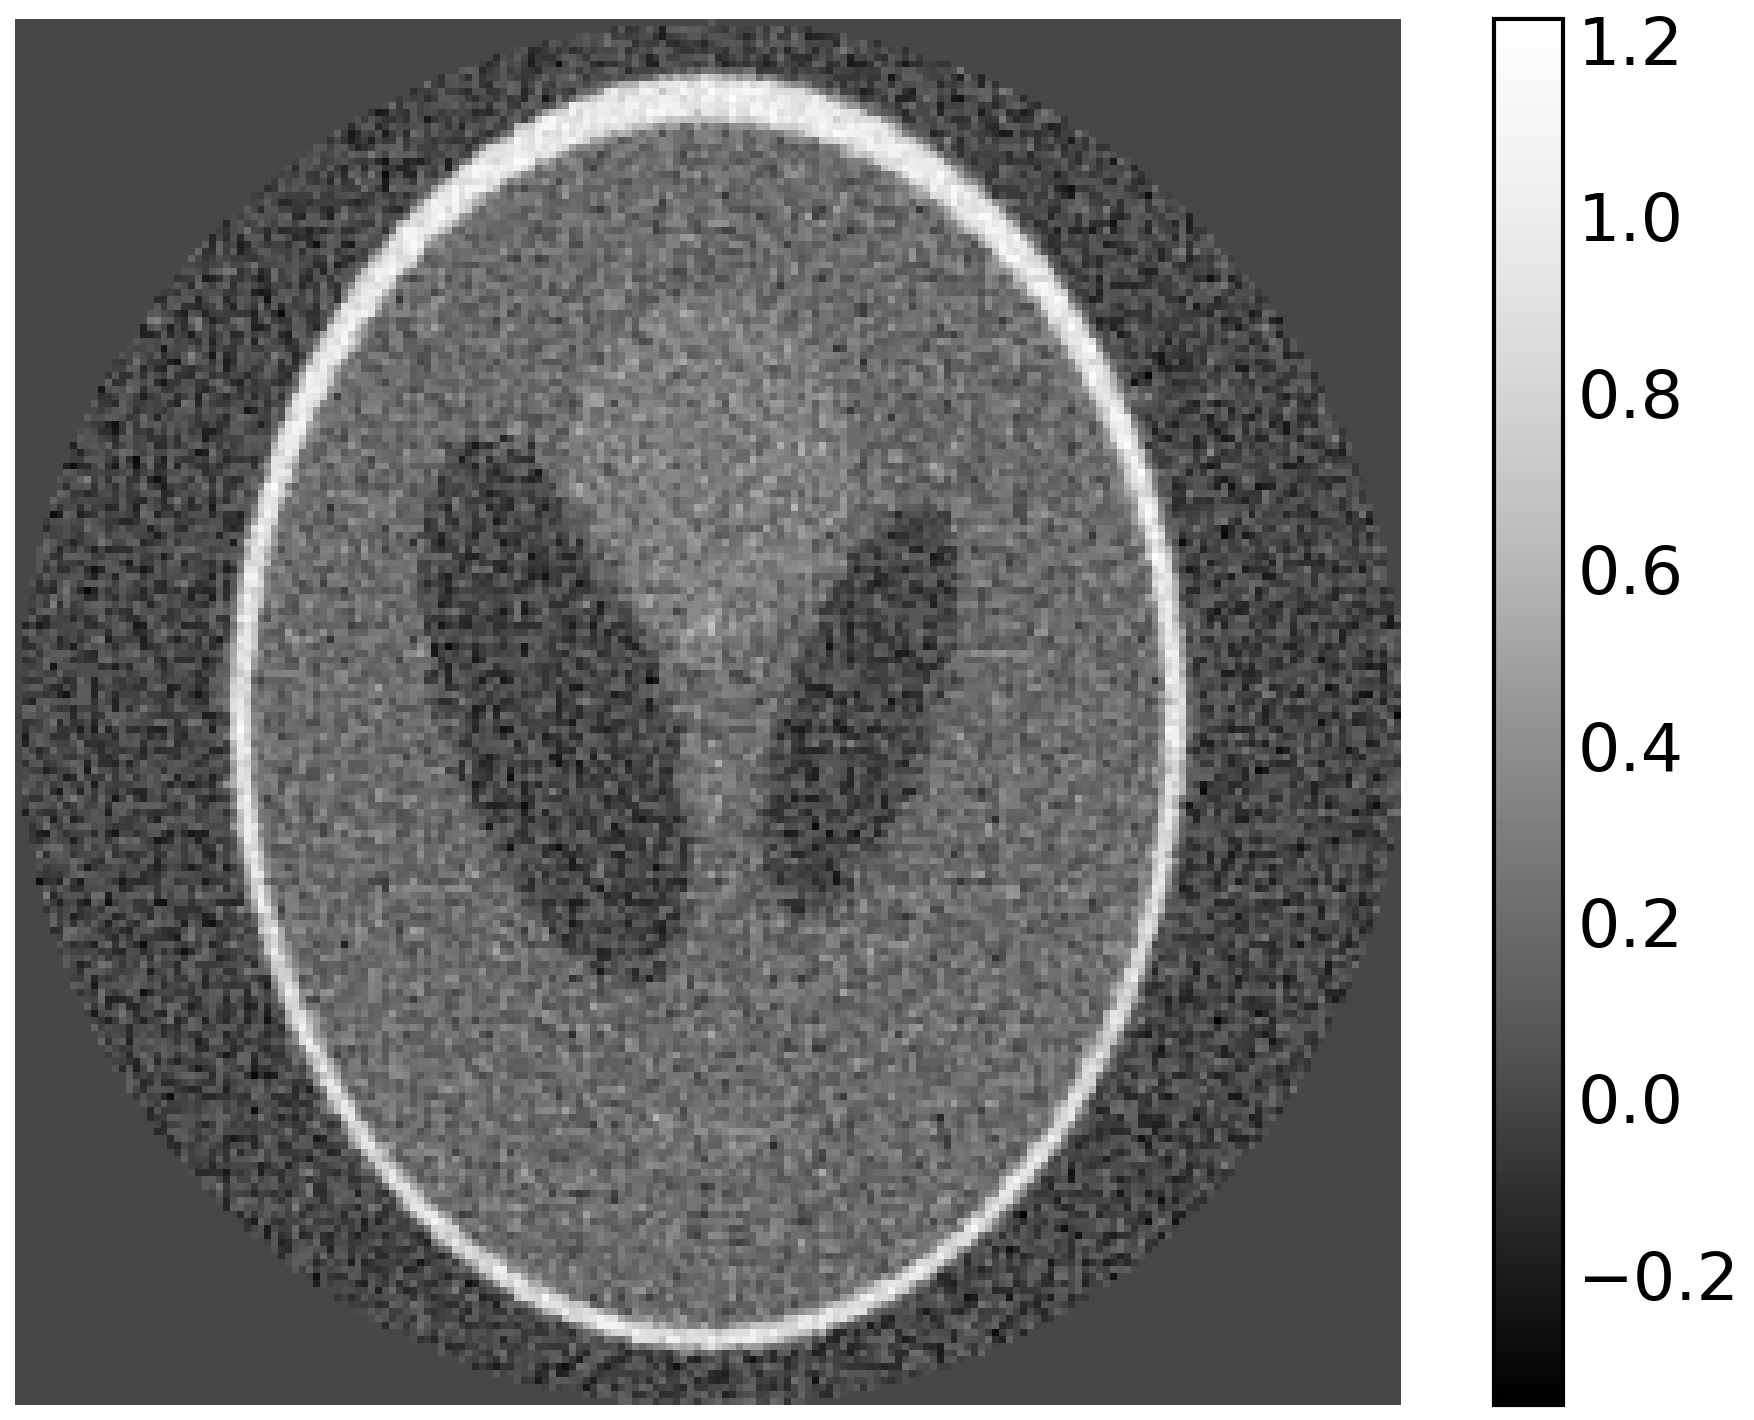
\includegraphics[width=0.24\textwidth]{images/ej_5/reconstruction_shepp_logan.png}\label{fig:fbp_shepp_logan_ej_5}}
    \hfill
    \caption{(a) fantoma original de \textit{Shepp-Logan}. Fantomas de Shepp-Logan reconstruidos con los siguientes filtros: (b) Hann, (c) Ramp y (d) Shepp-Logan.}
    \label{fig:reconstruccion_ruido}
\end{figure}

% --------------- EJ 6 ---------------------
\subsection*{Ejercicio 6}
Se creó una imagen con fondo negro que contiene únicamente un círculo blanco de 5 píxeles de radio centrado en el origen (ver Figura \ref{fig:circle_ej_6}). La imagen, con dimensiones de $100\times100$ (equivalentes a 100 detectores), fue utilizada para generar proyecciones y posteriormente reconstruir la imagen mediante retroproyección, variando el número de proyecciones (8, 16, 32 y 64). Además, se compararon los efectos de la retroproyección sin filtro y con un filtro \textit{Ramp}. Los resultados de estas comparaciones se presentan en la Figura \ref{fig: res_ej_6}.

\begin{figure} [htbp]
    \centering
    \includegraphics*[width=0.5\textwidth]{./images/ej_6/circle.png}
    \caption{iamgen de $100\times100$ generada con un circulo en el centro de radio 5 pixeles}
    \label{fig:circle_ej_6}
\end{figure}

\begin{figure}[htbp]
    \centering
    \subfloat[]{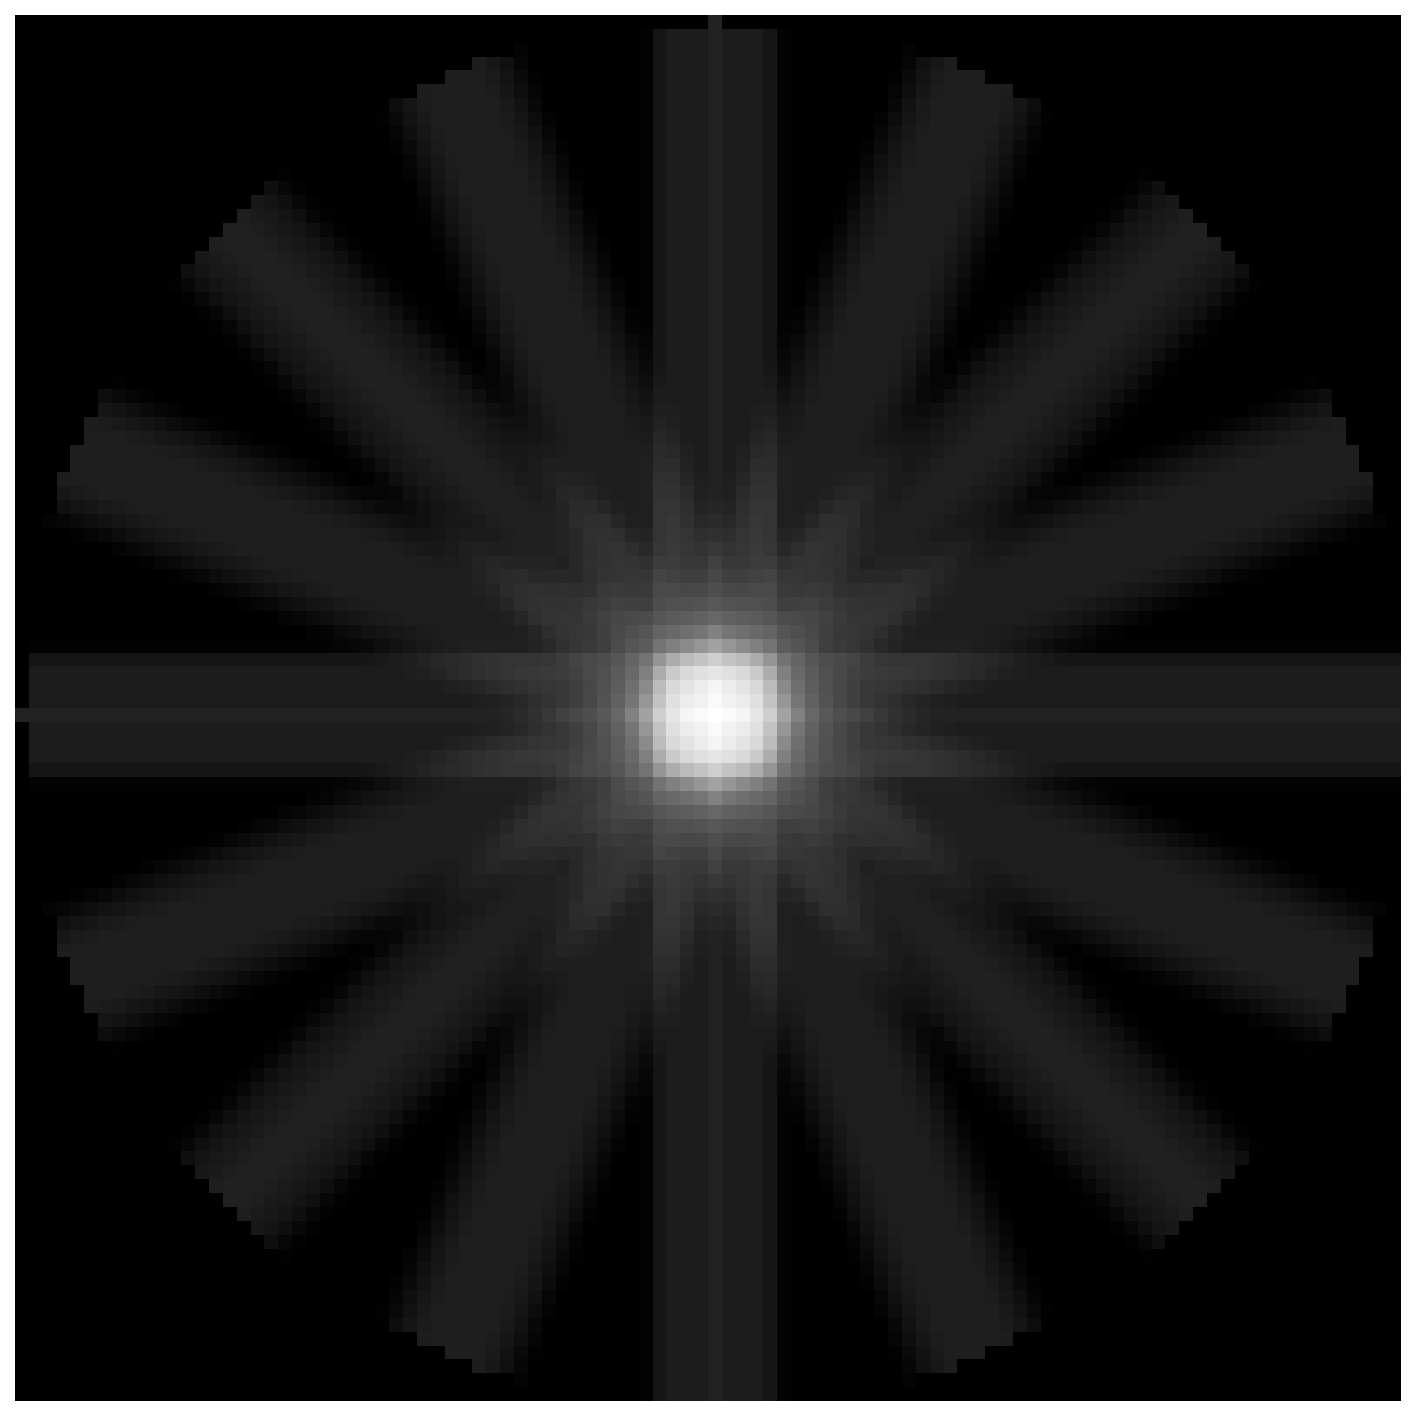
\includegraphics[width=0.24\textwidth]{images/ej_6/circle_none_8.png}\label{fig:fbp_circle_none_8}}
    \hfill
    \subfloat[]{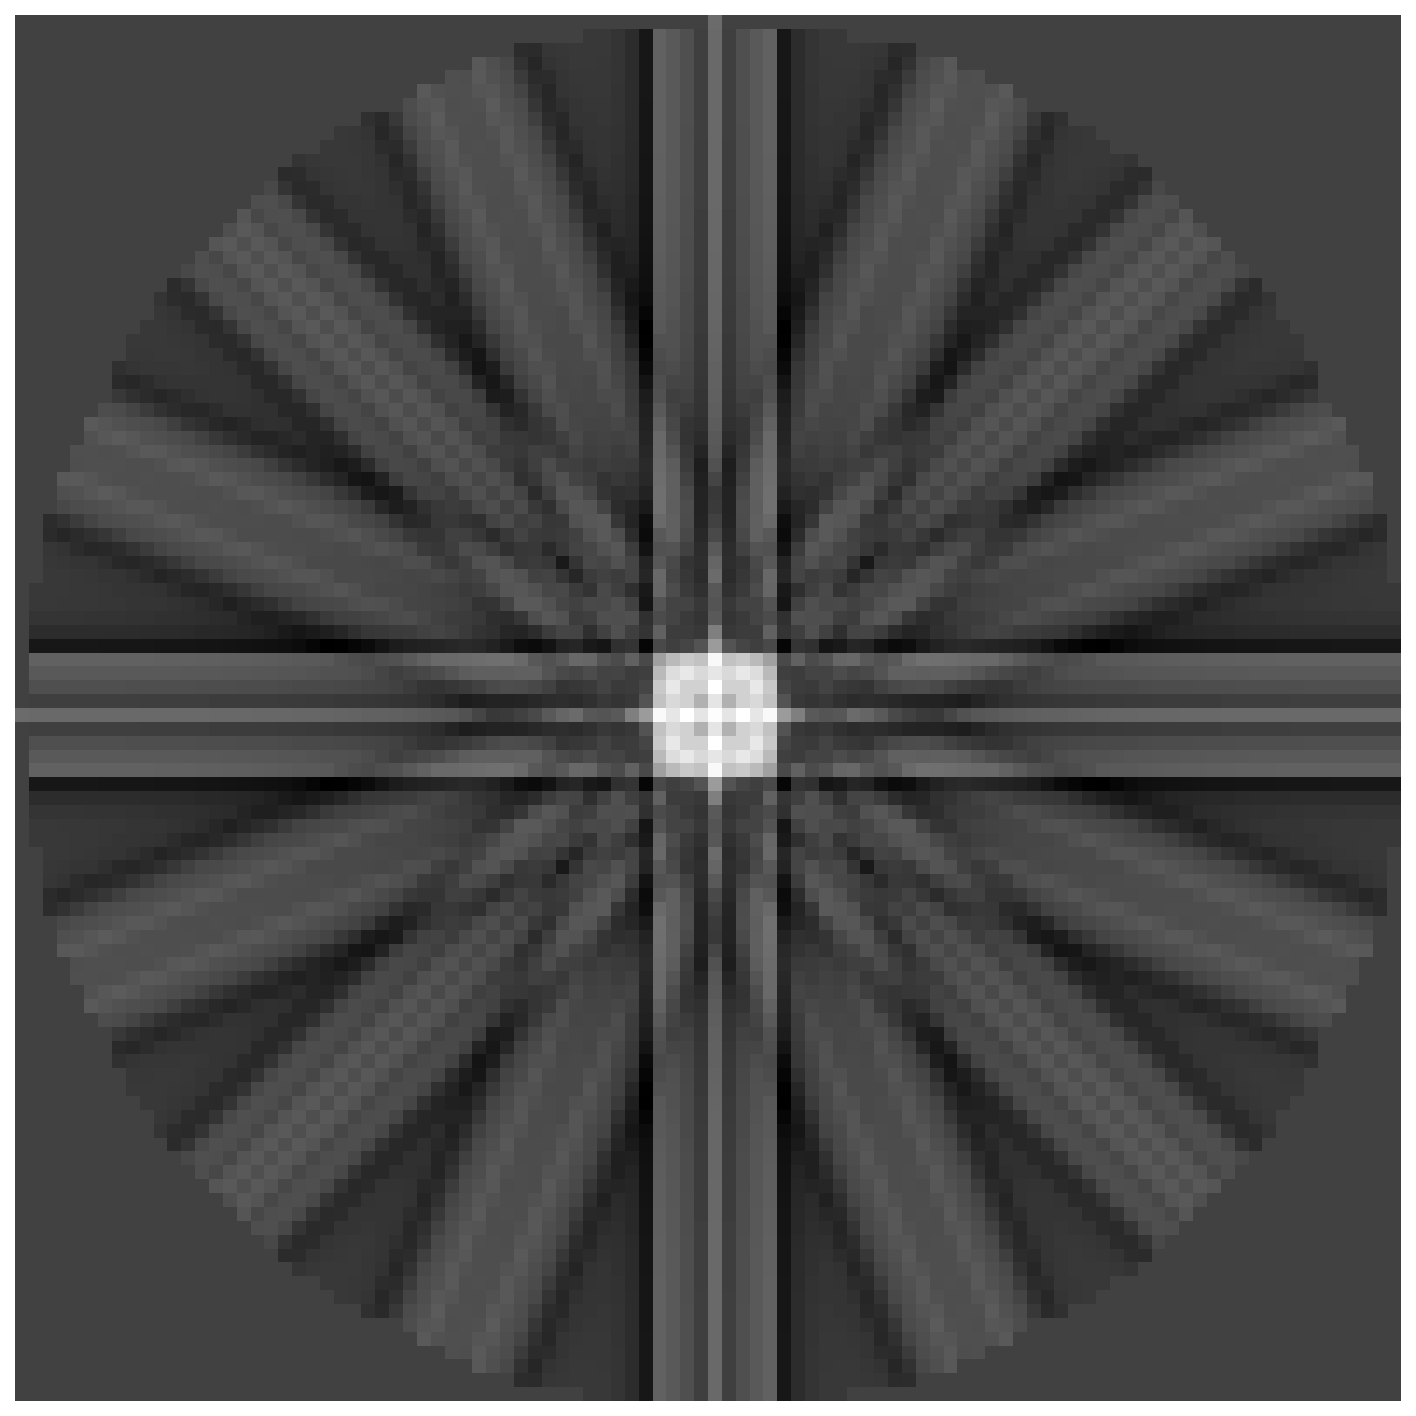
\includegraphics[width=0.24\textwidth]{images/ej_6/circle_ramp_8.png}\label{fig:fbp_circle_ramp_8}}
    \hfill
    \subfloat[]{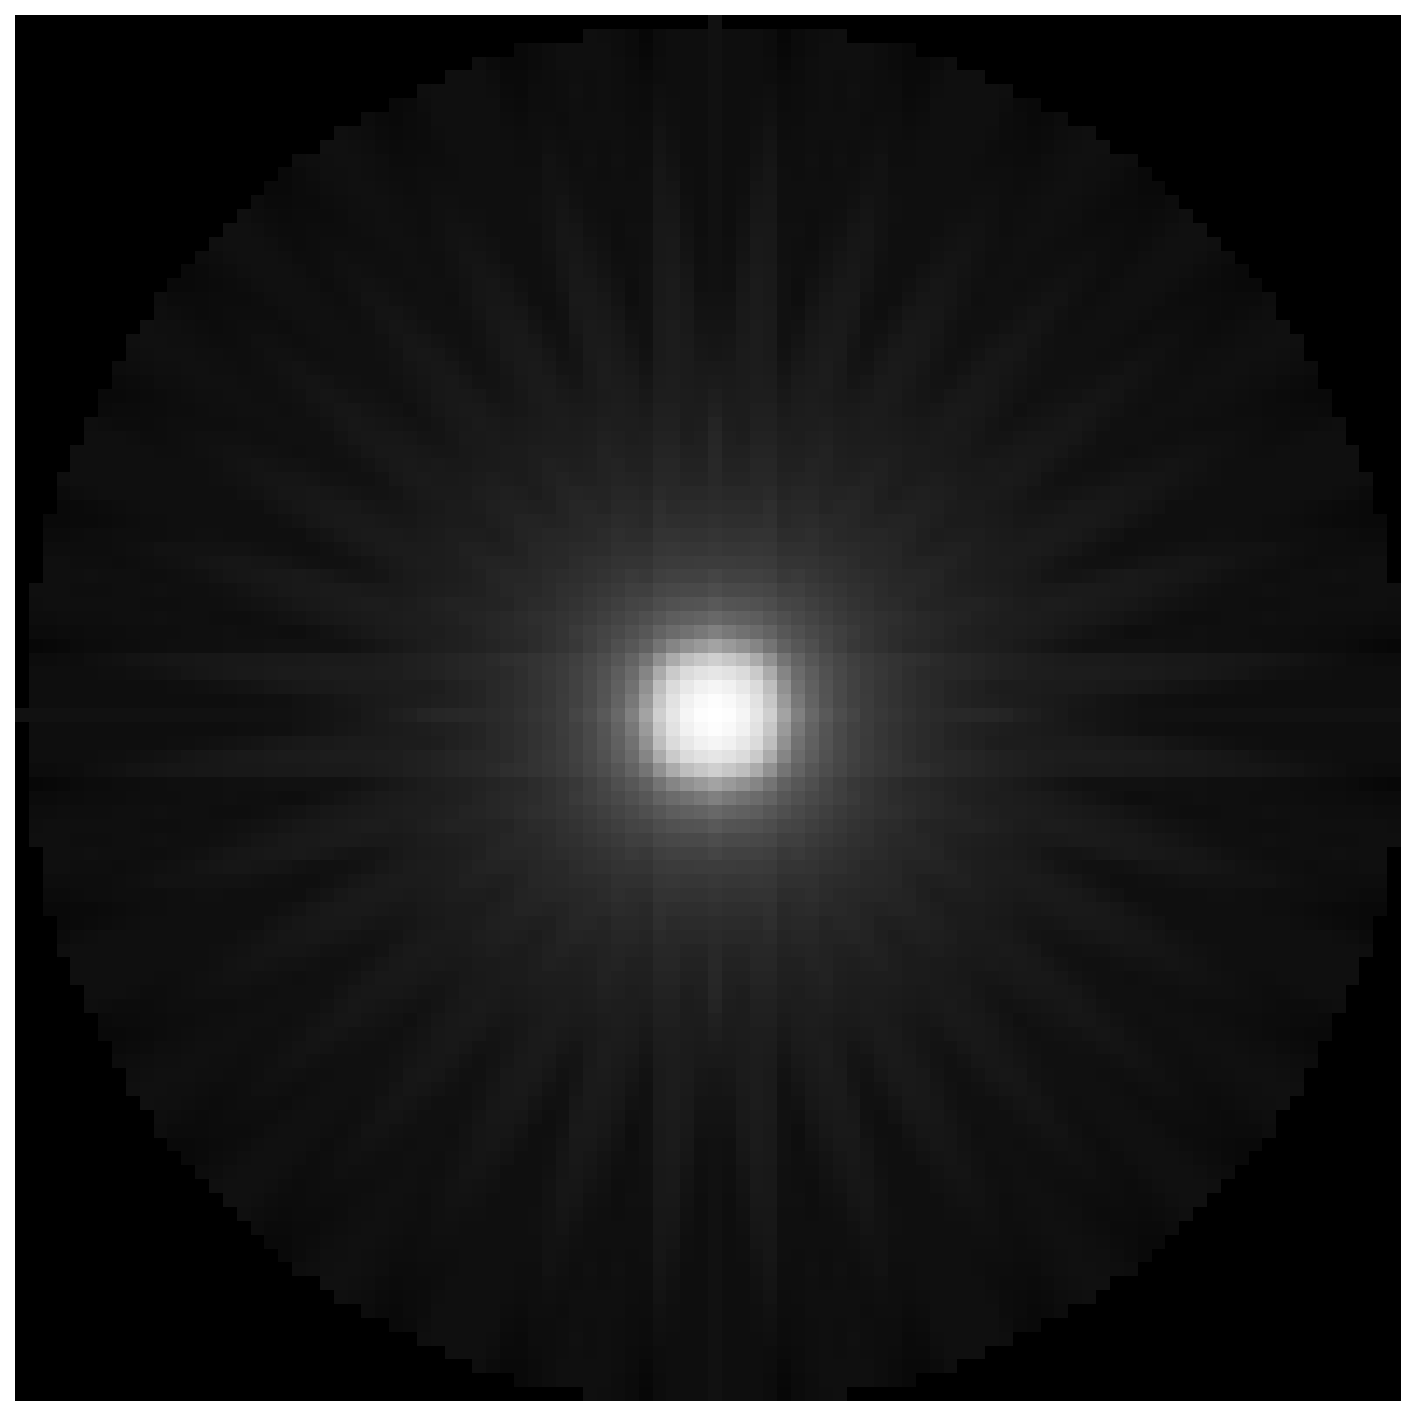
\includegraphics[width=0.24\textwidth]{images/ej_6/circle_none_16.png}\label{fig:fbp_circle_none_16}}
    \hfill
    \subfloat[]{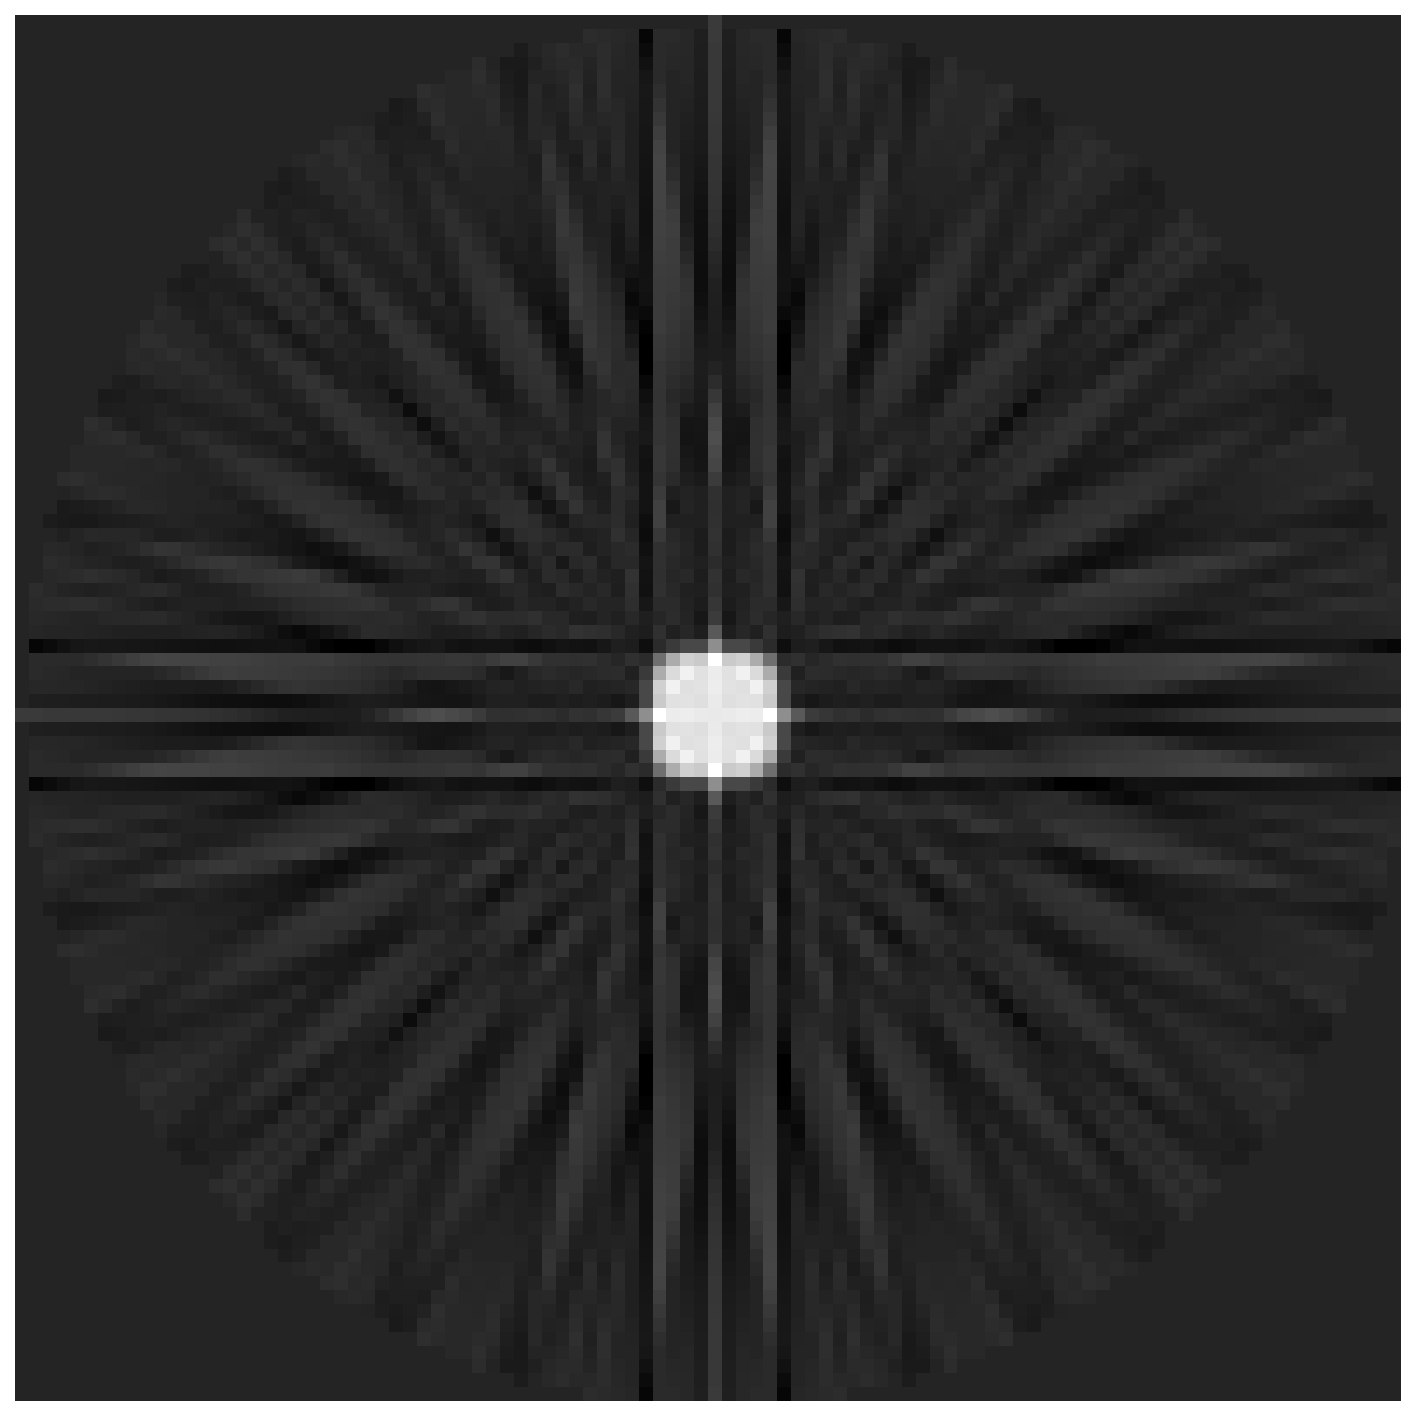
\includegraphics[width=0.24\textwidth]{images/ej_6/circle_ramp_16.png}\label{fig:fbp_circle_ramp_16}}
    \hfill
    \subfloat[]{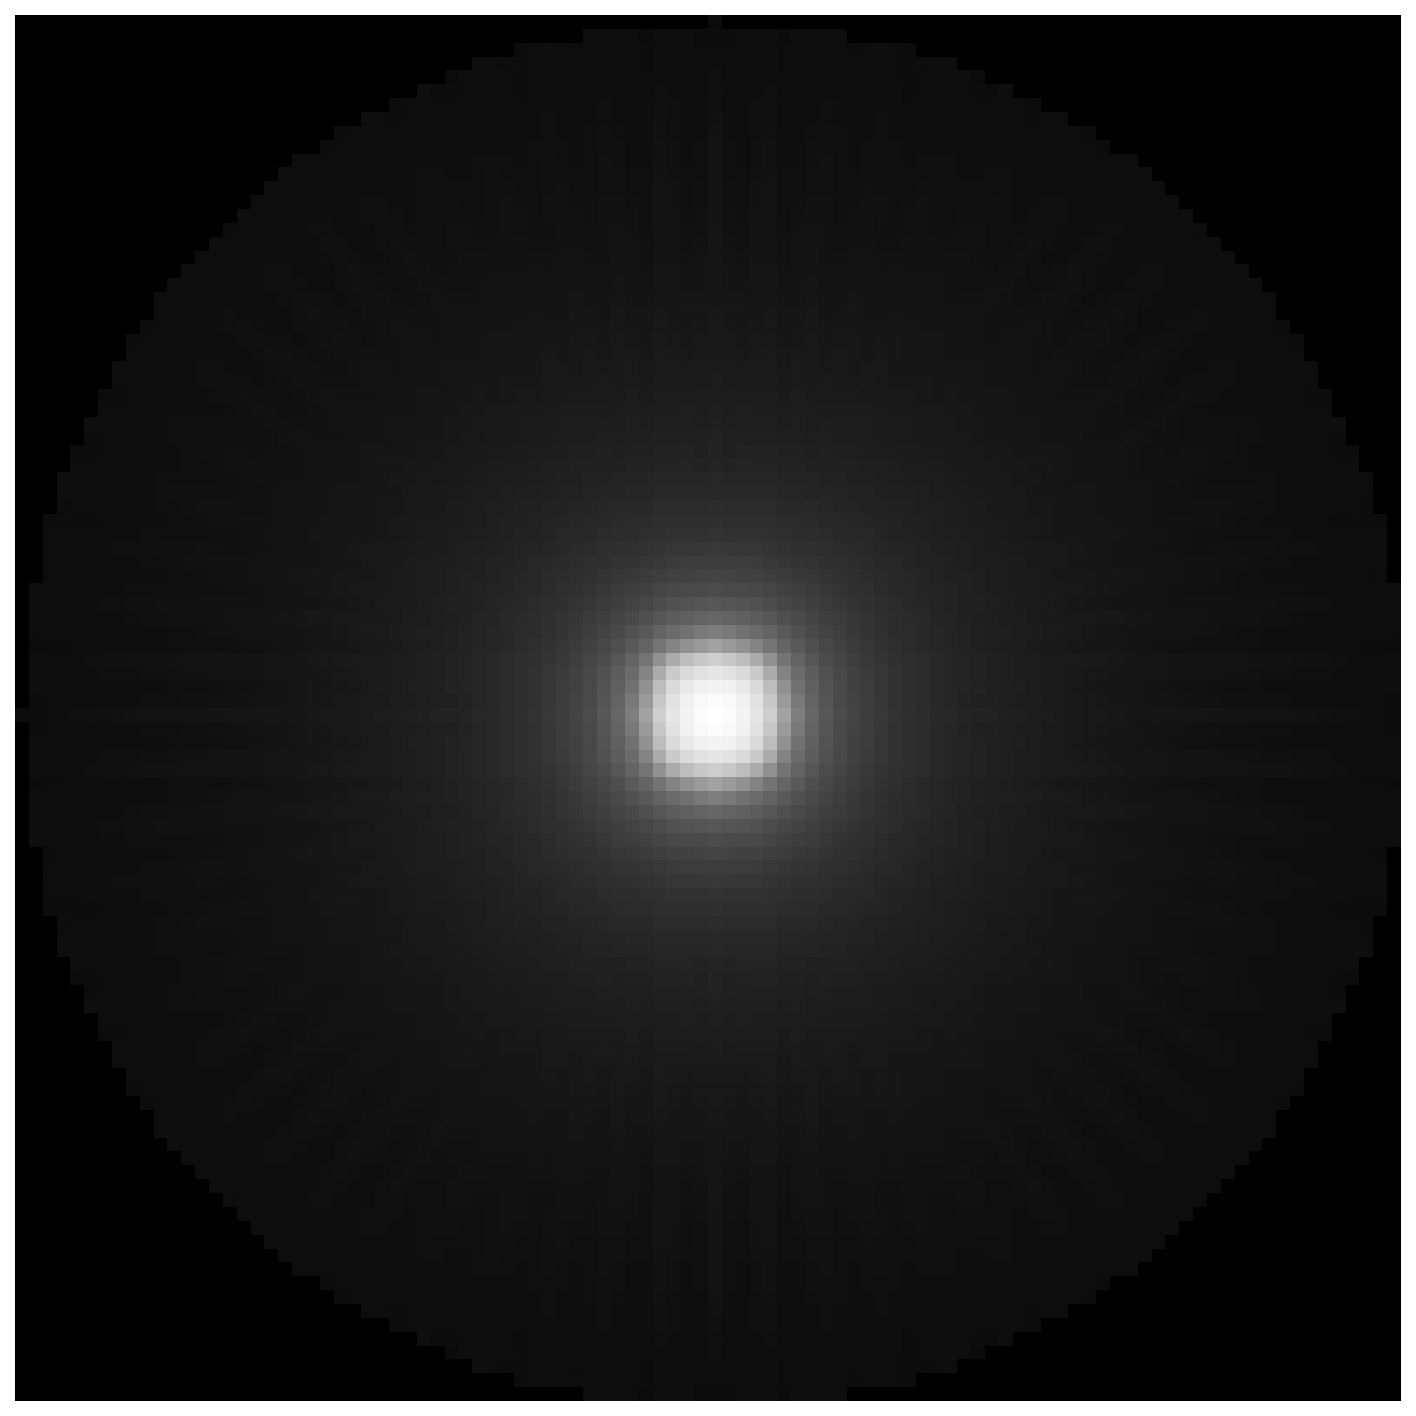
\includegraphics[width=0.24\textwidth]{images/ej_6/circle_none_32.png}\label{fig:fbp_circle_none_32}}
    \hfill
    \subfloat[]{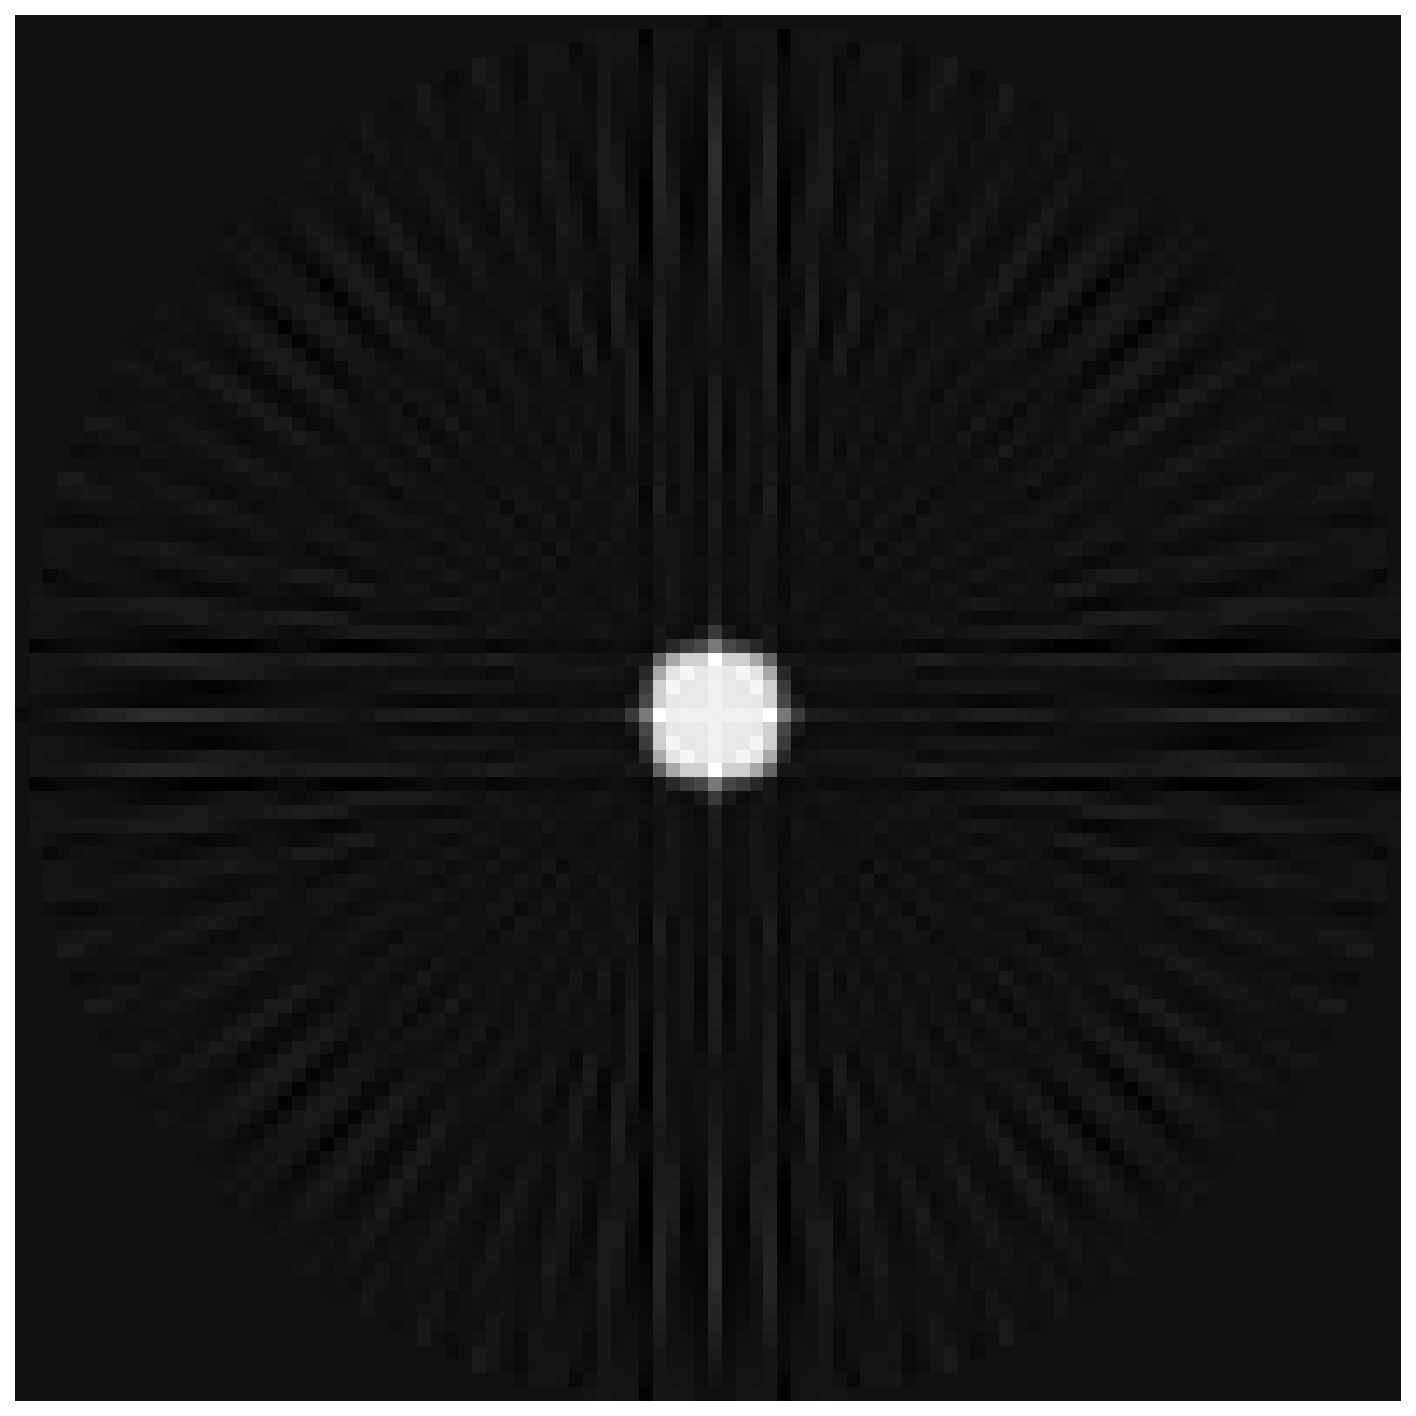
\includegraphics[width=0.24\textwidth]{images/ej_6/circle_ramp_32.png}\label{fig:fbp_circle_ramp_32}}
    \hfill
    \subfloat[]{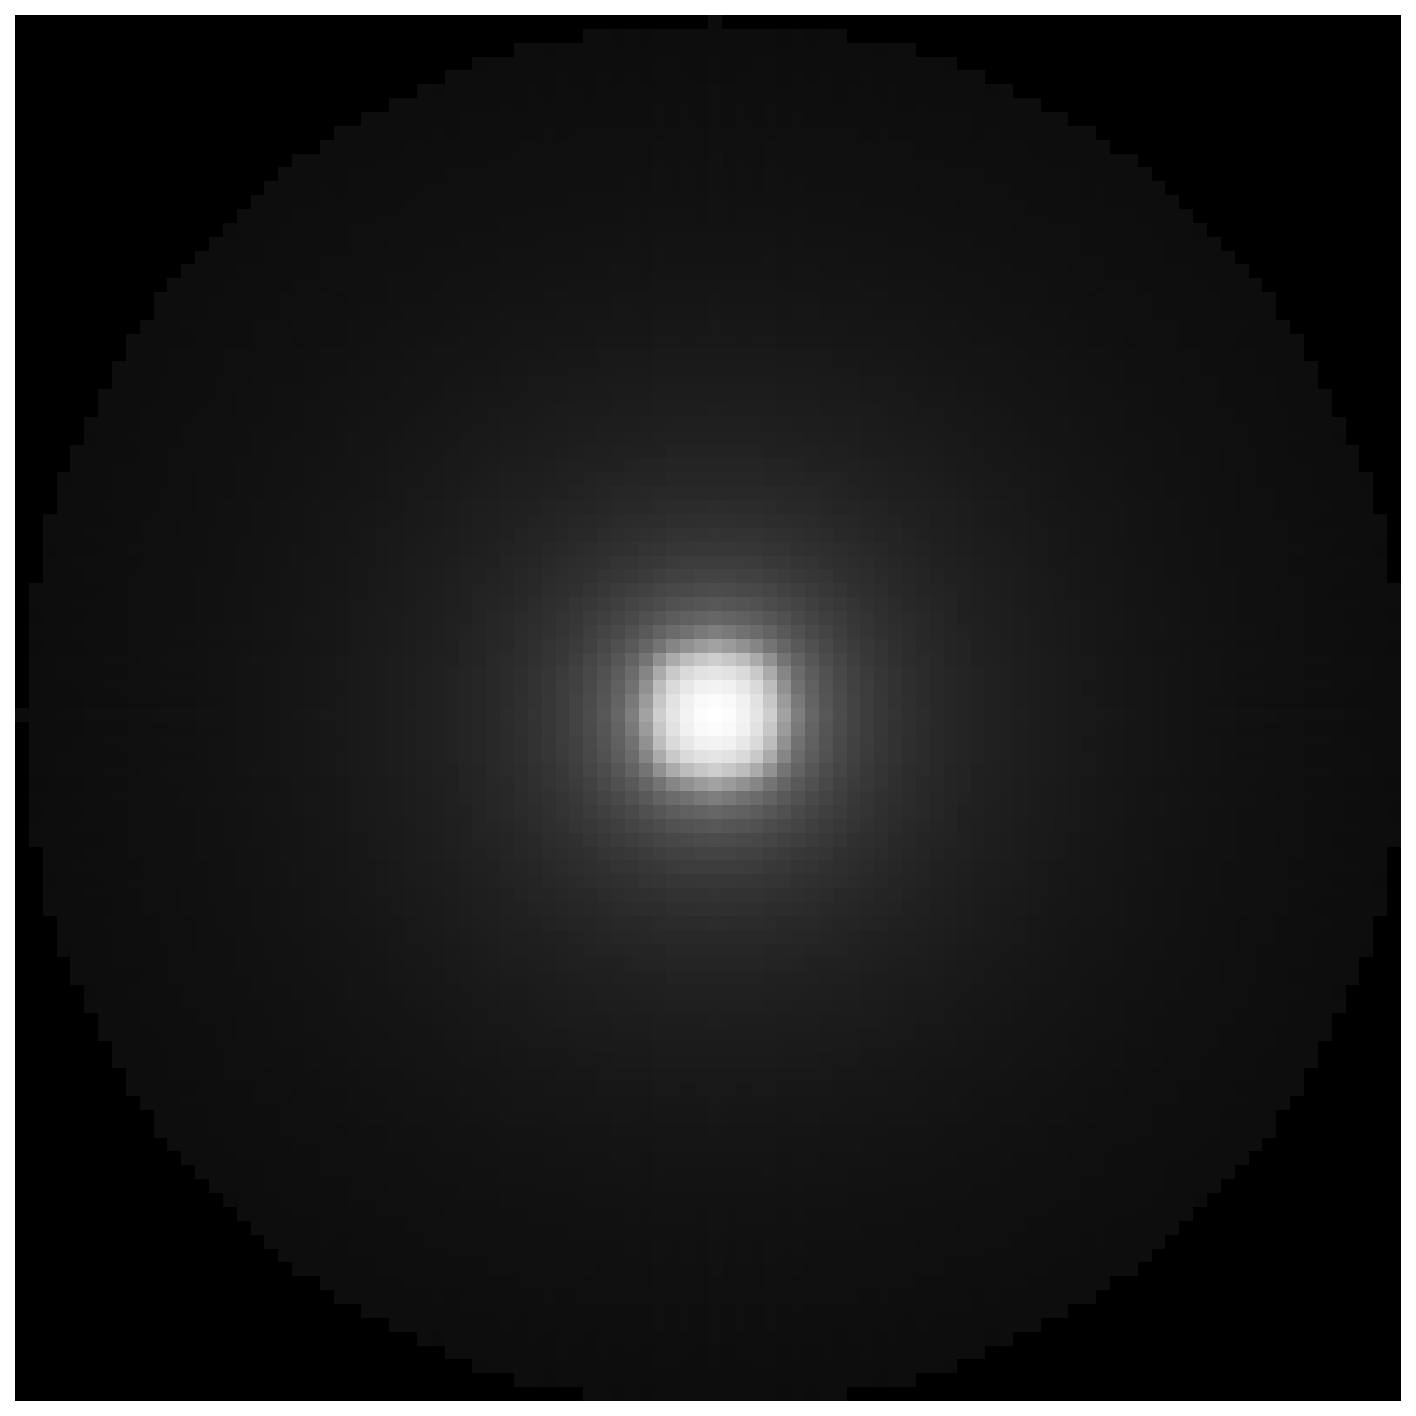
\includegraphics[width=0.24\textwidth]{images/ej_6/circle_none_64.png}\label{fig:fbp_circle_none_64}}
    \hfill
    \subfloat[]{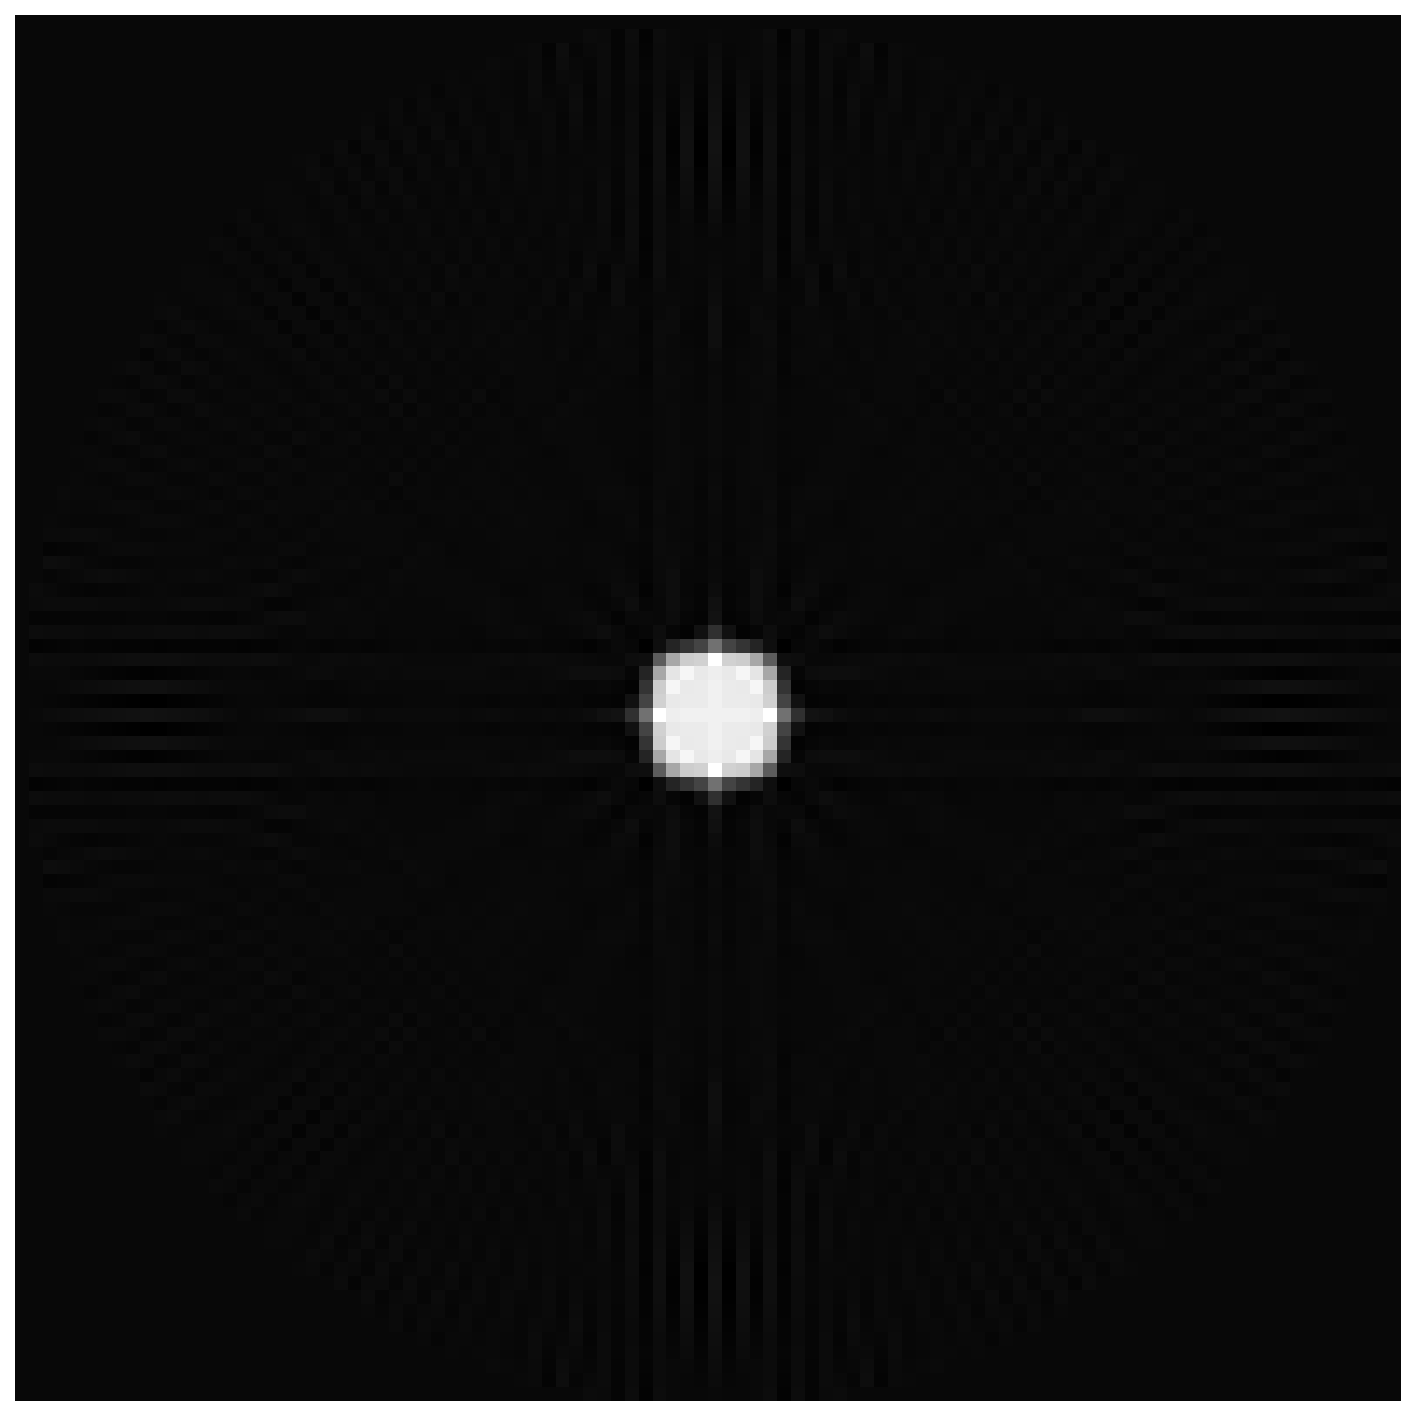
\includegraphics[width=0.24\textwidth]{images/ej_6/circle_ramp_64.png}\label{fig:fbp_circle_ramp_64}}
    \hfill
    \caption{Imagen reconstruida con retroproyección sin filtro (a, c, e, g) y con filtro \textit{Ramp} (b, d, f, h) para 8 (a, b), 16 (c, d), 32 (e, f) y 64 (g, h) proyecciones.}
    \label{fig: res_ej_6}
\end{figure}

En la Figura \ref{fig: res_ej_6} se observa que la reconstrucción de la imagen con retroproyección sin filtro produce artefactos en la imagen, como si esta se difuminara, independientemente del número de proyecciones. Por otro lado, la reconstrucción con filtro \textit{Ramp} produce una imagen más nítida y con menos artefactos, aunque todavía se observan artefactos en la imagen reconstruida con 8 y 16 proyecciones. A medida que el número de proyecciones aumenta, la calidad de la imagen reconstruida mejora, y los artefactos se reducen.

% --------------- EJ 7 ---------------------
\subsection*{Ejercicio 7}
En este ejercicio, se simuló la situación en que un detector falla. Esta falla produce una linea negra en el sinograma, para un valor especifico de $x'$ (posición del detector) y para todos los ángulos $\theta$. Se generó el sinograma del fantoma de \textit{Shepp-Logan} con 120 ángulos $\theta$ equiespaciados entre 0 y 180 grados, y se introdujo una falla en el detector 80. El sinograma resultante se muestra en la Figura \ref{fig:sinograma_falla}.

\begin{figure}
    \centering
    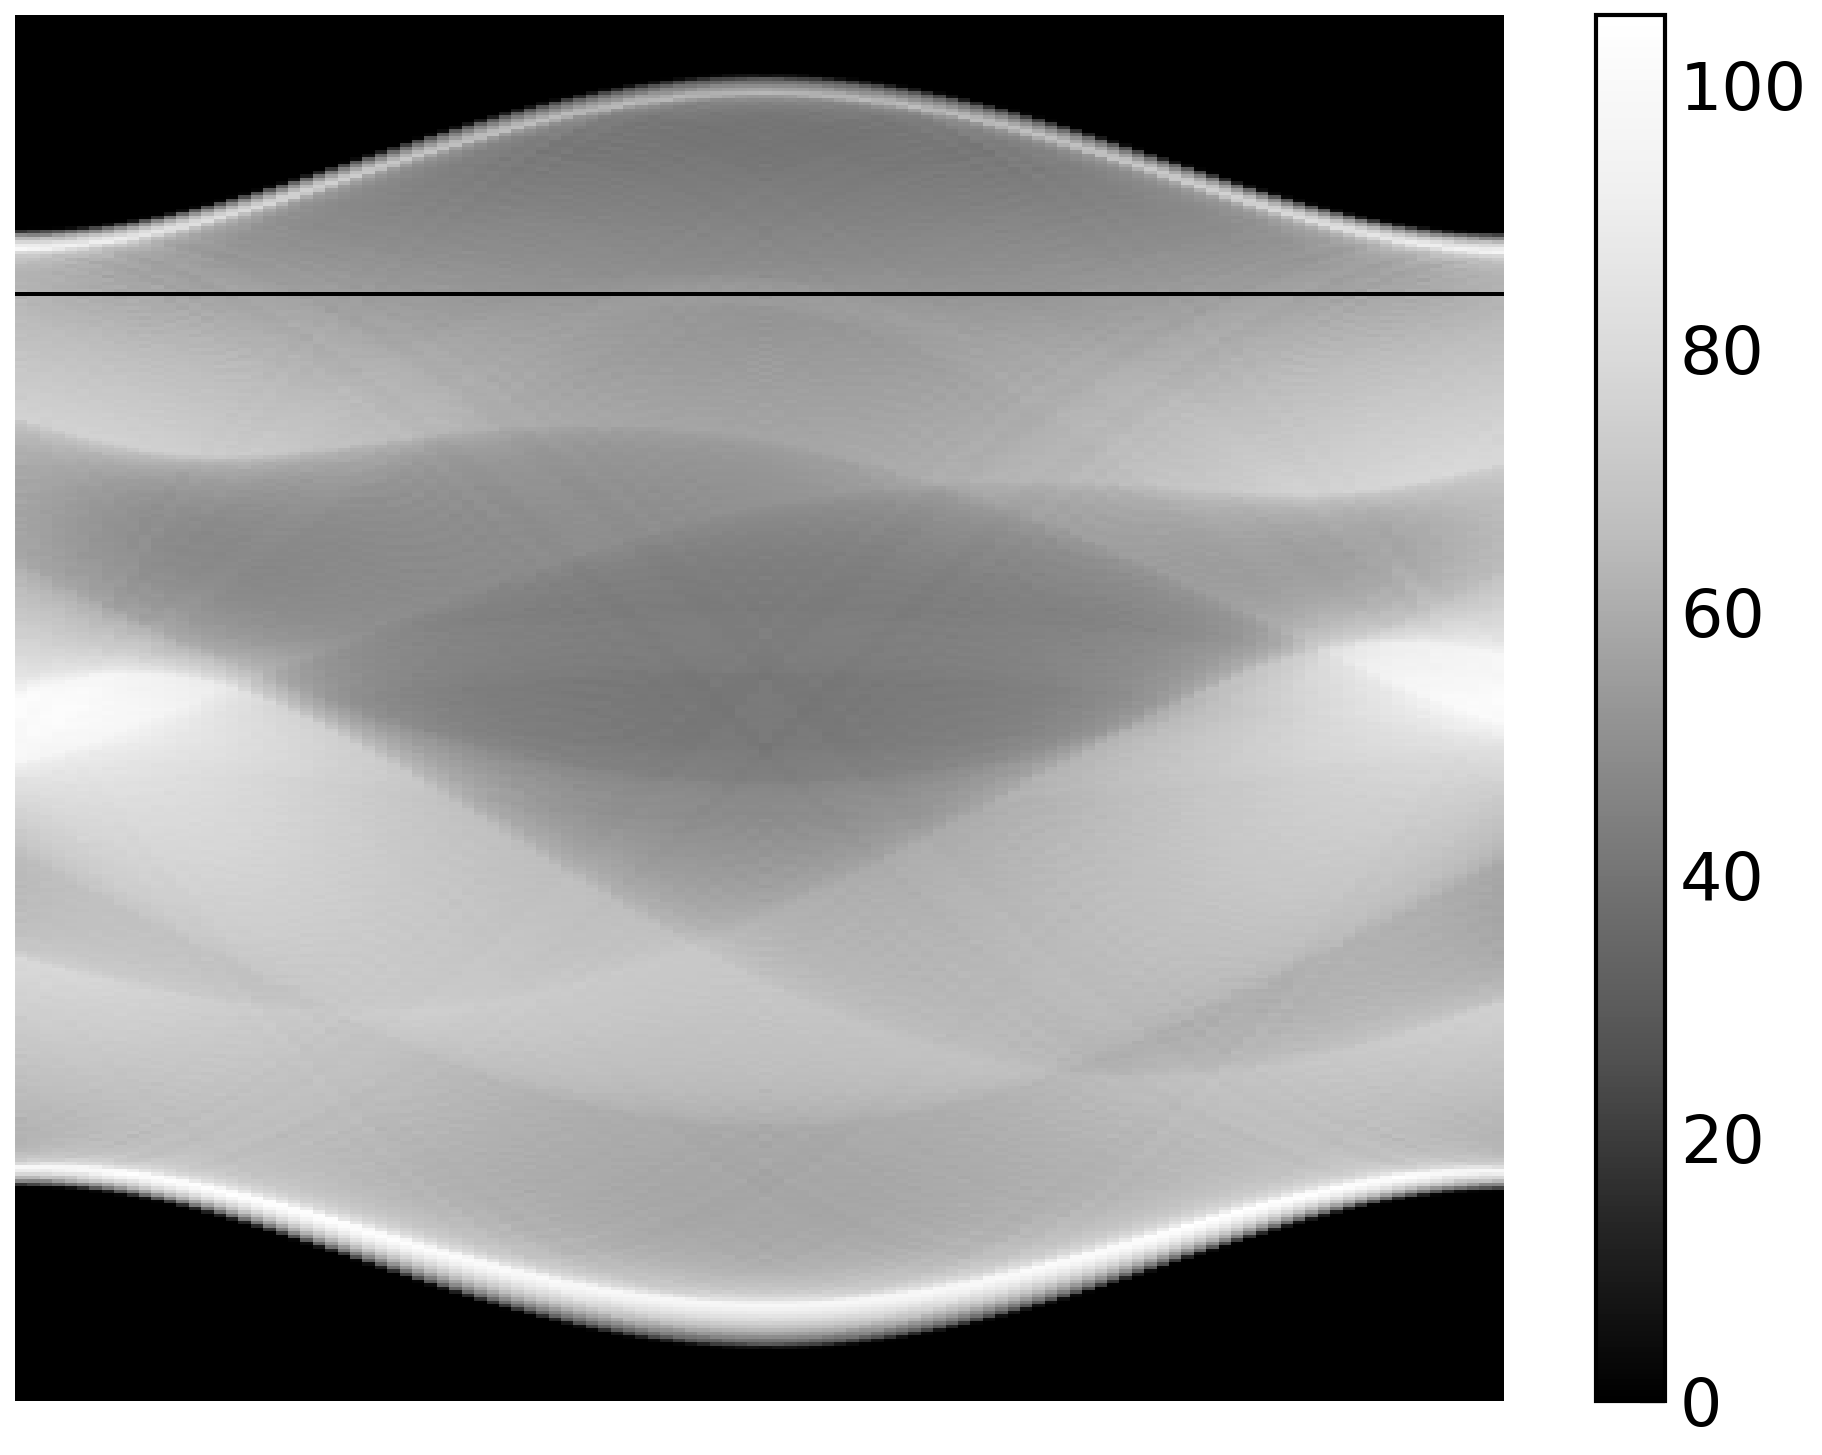
\includegraphics[width=0.5\textwidth]{images/ej_7/sinogram_line.png}
    \caption{sinograma del fantoma de \textit{Shepp-Logan} con una falla en el detector 80.}
    \label{fig:sinograma_falla}
\end{figure}

Se realizó la reconstrucción de la imagen a partir del sinograma con la falla en el detector 80, utilizando el algoritmo de retroproyección filtrada con el filtro \textit{Hann}. El resultado se muestra en la Figura \ref{fig:reconstruccion_falla}.

\begin{figure}
    \centering
    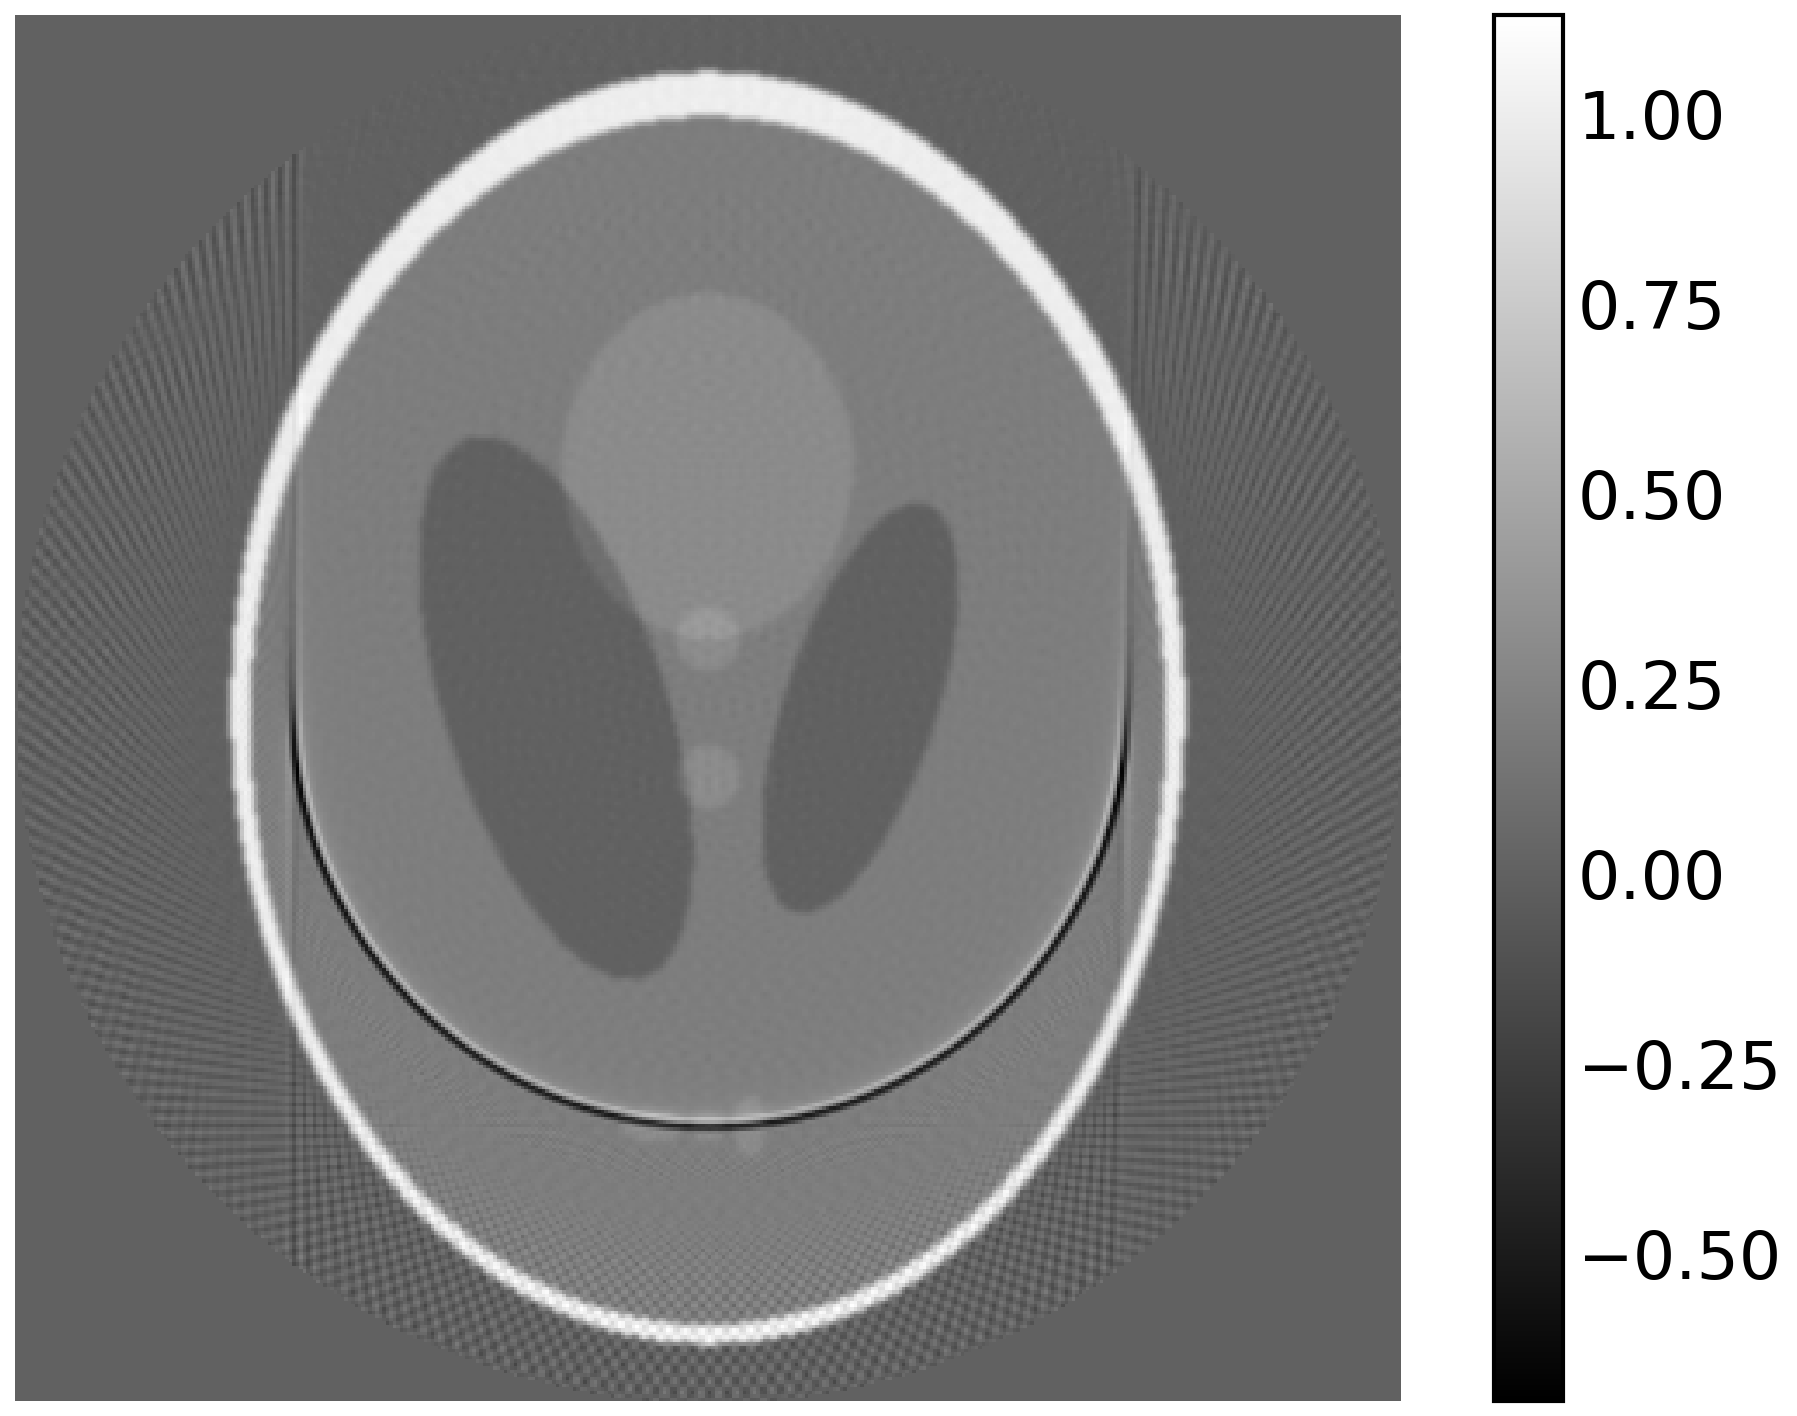
\includegraphics[width=0.5\textwidth]{images/ej_7/reconstruction_line.png}
    \caption{reconstrucción de la imagen a partir del sinograma con una falla en el detector 80.}
    \label{fig:reconstruccion_falla}
\end{figure}

En la Figura \ref{fig:reconstruccion_falla}, se evidencia que la reconstrucción de la imagen, basada en el sinograma con la falla en el detector 80, genera artefactos notables, representados por líneas negras con forma de anillos. Asimismo, la reconstrucción provoca una atenuación en comparación con la imagen original.

% ------------------ CONCLUSION ---------------------
\section{Conclusiones}


\end{document}
